%===============================================================================
% LaTeX sjabloon voor de bachelorproef toegepaste informatica aan HOGENT
% Meer info op https://github.com/HoGentTIN/latex-hogent-report
%===============================================================================

\documentclass[dutch,dit,thesis]{hogentreport}

% TODO:
% - If necessary, replace the option `dit`' with your own department!
%   Valid entries are dbo, dbt, dgz, dit, dlo, dog, dsa, soa
% - If you write your thesis in English (remark: only possible after getting
%   explicit approval!), remove the option "dutch," or replace with "english".

\usepackage{lipsum} % For blind text, can be removed after adding actual content

%% Pictures to include in the text can be put in the graphics/ folder
\graphicspath{{graphics/}}

%% For source code highlighting, requires pygments to be installed
%% Compile with the -shell-escape flag!
\usepackage[section]{minted}
\usepackage{comment}
\usemintedstyle{solarized-light}
\definecolor{bg}{RGB}{253,246,227} %% Set the background color of the codeframe

%% Change this line to edit the line numbering style:
\renewcommand{\theFancyVerbLine}{\ttfamily\scriptsize\arabic{FancyVerbLine}}

%% Macro definition to load external java source files with \javacode{filename}:
\newmintedfile[javacode]{java}{
    bgcolor=bg,
    fontfamily=tt,
    linenos=true,
    numberblanklines=true,
    numbersep=5pt,
    gobble=0,
    framesep=2mm,
    funcnamehighlighting=true,
    tabsize=4,
    obeytabs=false,
    breaklines=true,
    mathescape=false
    samepage=false,
    showspaces=false,
    showtabs =false,
    texcl=false,
}

% Other packages not already included can be imported here

%%---------- Document metadata -------------------------------------------------
% TODO: Replace this with your own information
\author{Ernst Aarden}
\supervisor{Dhr. F. Van Houte}
\cosupervisor{Mevr. S. Beeckman}
\title[Optionele ondertitel]%
    {Titel van de bachelorproef}
\academicyear{\advance\year by -1 \the\year--\advance\year by 1 \the\year}
\examperiod{1}
\degreesought{\IfLanguageName{dutch}{Professionele bachelor in de toegepaste informatica}{Bachelor of applied computer science}}
\partialthesis{false} %% To display 'in partial fulfilment'
%\institution{Internshipcompany BVBA.}

%% Add global exceptions to the hyphenation here
\hyphenation{back-slash}

%% The bibliography (style and settings are  found in hogentthesis.cls)
\addbibresource{bachproef.bib}            %% Bibliography file
\addbibresource{../voorstel/voorstel.bib} %% Bibliography research proposal
\defbibheading{bibempty}{}

%% Prevent empty pages for right-handed chapter starts in twoside mode
\renewcommand{\cleardoublepage}{\clearpage}

\renewcommand{\arraystretch}{1.2}

%% Content starts here.
\begin{document}

%---------- Front matter -------------------------------------------------------

\frontmatter

\hypersetup{pageanchor=false} %% Disable page numbering references
%% Render a Dutch outer title page if the main language is English
\IfLanguageName{english}{%
    %% If necessary, information can be changed here
    \degreesought{Professionele Bachelor toegepaste informatica}%
    \begin{otherlanguage}{dutch}%
       \maketitle%
    \end{otherlanguage}%
}{}

%% Generates title page content
\maketitle
\hypersetup{pageanchor=true}

%%=============================================================================
%% Voorwoord
%%=============================================================================

\chapter*{Woord vooraf}%
\label{ch:voorwoord}

% TODO: OK?
%% Het voorwoord is het enige deel van de bachelorproef waar je vanuit je
%% eigen standpunt (``ik-vorm'') mag schrijven. Je kan hier bv. motiveren
%% waarom jij het onderwerp wil bespreken.
%% Vergeet ook niet te bedanken wie je geholpen/gesteund/... heeft

Deze scriptie werd geschreven in het kader van het voltooien van de opleiding Toegepaste Informatica in de specialisatie System \& Network Administrator. \\

Het onderwerp van de bachelorproef werd me aangereikt via mijn stagebedrijf Easi. In het specifiek door de heer Jarne Creten, die ook het co-promotorschap heeft opgenomen. Ik heb van in het begin steeds een grote interesse gehad in Microsoft-technologieën. Microsoft Graph leek me een geschikte kandidaat wanneer dit onderwerp tot me werd geïntroduceerd. De complexiteit en mogelijkheden van Microsoft Graph zorgde voor extra motivatie. Daarnaast ben ik ook gefascineerd door de cloud, hierdoor wou ik me volledig verdiepen tot dit onderwerp. \\

Voor de volgende personen wil ik graag een oprechte dankuwel uitdrukken. Zonder hun hulp, moeite, tijd en zoveel meer zou deze scriptie niet tot stand zijn gekomen. \\

Eerst en vooral wil ik mijn co-promotor, Jarne Creten, bedanken voor zijn rol in dit onderzoek. Hij heeft mij tot dit onderwerp geïntroduceerd. Daarnaast kon ik dag en nacht bij hem terecht voor elk obstakel dat in mijn weg lag. Hij gaf me steeds de juiste feedback en wou dat dit onderzoek een succes zou worden. \\

Als tweede wil ik mijn promotor, Gertjan Bosteels, bedanken voor zijn sturing tijdens dit uitwerkingsproces. Hij gaf me de feedback die ik nodig had en stond steeds klaar om mijn vragen te beantwoorden. \\

Ook wil ik de mede-studenten van mijn academiejaar bedanken voor hun feedback. Bij elke vraag wouden ze mee naar een antwoord zoeken. \\

Als laatste wil ik mijn familie en vrienden bedanken. Sinds de start van mijn opleiding stonden ze steeds klaar voor mij. Het was een enorme mentale steun om te weten dat zij steeds in mij geloofden. \\

Ik wens u van harte een leuke en boeiende leeservaring toe!


% !TeX spellcheck = nl_NL-Dutch
%%=============================================================================
%% Samenvatting
%%=============================================================================

% TODO: De "abstract" of samenvatting is een kernachtige (~ 1 blz. voor een thesis) synthese van het document.
%
% Een goede abstract biedt een kernachtig antwoord op volgende vragen:
%
% 1. Waarover gaat de bachelorproef?
% 2. Waarom heb je er over geschreven?
% 3. Hoe heb je het onderzoek uitgevoerd?
% 4. Wat waren de resultaten? Wat blijkt uit je onderzoek?
% 5. Wat betekenen je resultaten? Wat is de relevantie voor het werkveld?
%
% Daarom bestaat een abstract uit volgende componenten:
%
% - inleiding + kaderen thema
% - probleemstelling
% - (centrale) onderzoeksvraag
% - onderzoeksdoelstelling
% - methodologie
% - resultaten (beperk tot de belangrijkste, relevant voor de onderzoeksvraag)
% - conclusies, aanbevelingen, beperkingen
% === SAMENVATTING ===
%\IfLanguageName{english}{%
\selectlanguage{dutch}
\chapter*{Samenvatting}
Deze scriptie onderzoekt de evolutie van Azure Active Directory Graph naar Microsoft Graph binnen het domein van Microsoft administration. Het bedrijf Easi maakt gebruik van de uitfaserende Azure Active Directory Graph en wil weten of Microsoft Graph klaar is om deze uitfaserende technologie te vervangen. Het doel van het onderzoek is om te bepalen of Microsoft Graph op dit moment instaat is om de beheertaken die eerder mogelijk waren met Azure Active Directory Graph over te nemen. Naast het beantwoorden van deze vraag, zijn de onderzoeksdoelstellingen het herwerken van een PowerShell-script met Microsoft Graph en het vergroten van de kennis over Microsoft Graph voor Microsoft-systeembeheerders. De methodologie van het onderzoek bestaat uit twee delen. In eerste instantie wordt een vergelijkende studie uitgevoerd op basis van vier criteria om Azure Active Directory Graph en Microsoft Graph te analyseren. Vervolgens wordt een Proof-of-Concept gerealiseerd door middel van het herschrijven van een PowerShell-script met behulp van Microsoft Graph PowerShell-modules. De resultaten van het onderzoek tonen aan dat 11 van de 20 functies volledig kunnen worden herwerkt en twee functies deels zijn herwerkt. De resterende zeven functies zijn omtrent niet-persoonlijke mailboxen en kunnen niet worden omgezet, wat leidt tot limitaties van de technologie vandaag de dag. Daarnaast concludeert de vergelijkende studie dat beide technologieën gelijkenissen vertonen, maar toch verschillen op eindpunt, aanspreekbare data-objecten en dependencies. De resultaten van beide delen tonen aan dat Microsoft Graph nog niet volledig in staat is om de beheertaken van Azure Active Directory Graph over te nemen. Op basis van de resultaten wordt volgende conclusie getrokken. Het blijkt dat Microsoft Graph verdergaat dan enkel het vervangen van Azure Active Directory Graph. Azure Active Directory Graph is gefocust op het beheren van Azure Active Directory, terwijl Microsoft Graph vandaag de dag ook Microsoft Teams, Outlook en andere Microsoft-entiteiten kan beheren. 

%\selectlanguage{english}

%%---------- Samenvatting -----------------------------------------------------
% De samenvatting in de hoofdtaal van het document

% Azure \ac{AD} is gefocust op het beheren van Azure \ac{AD}, terwijl Microsoft Graph vandaag de dag ook Microsoft Teams, Outlook, To Do en andere entiteiten kan aanspreken naast Azure \ac{AD}. Azure \ac{AD} kan minder Microsoft-entiteiten aanspreken in vergelijking met Microsoft Graph. 


%---------- Inhoud, lijst figuren, ... -----------------------------------------

\tableofcontents

% In a list of figures, the complete caption will be included. To prevent this,
% ALWAYS add a short description in the caption!
%
%  \caption[short description]{elaborate description}
%
% If you do, only the short description will be used in the list of figures

\listoffigures

% If you included tables and/or source code listings, uncomment the appropriate
% lines.
%\listoftables
%\listoflistings

% Als je een lijst van afkortingen of termen wil toevoegen, dan hoort die
% hier thuis. Gebruik bijvoorbeeld de ``glossaries'' package.
% https://www.overleaf.com/learn/latex/Glossaries

%---------- Kern ---------------------------------------------------------------

\mainmatter{}

% De eerste hoofdstukken van een bachelorproef zijn meestal een inleiding op
% het onderwerp, literatuurstudie en verantwoording methodologie.
% Aarzel niet om een meer beschrijvende titel aan deze hoofdstukken te geven of
% om bijvoorbeeld de inleiding en/of stand van zaken over meerdere hoofdstukken
% te verspreiden!

%%=============================================================================
%% Inleiding
%%=============================================================================

\chapter{\IfLanguageName{dutch}{Inleiding}{Introduction}}%
\label{ch:inleiding}

\begin{comment}
De inleiding moet de lezer net genoeg informatie verschaffen om het onderwerp te begrijpen en in te zien waarom de onderzoeksvraag de moeite waard is om te onderzoeken. In de inleiding ga je literatuurverwijzingen beperken, zodat de tekst vlot leesbaar blijft. Je kan de inleiding verder onderverdelen in secties als dit de tekst verduidelijkt. Zaken die aan bod kunnen komen in de inleiding~\autocite{Pollefliet2011}:

\begin{itemize}
  \item context, achtergrond
  \item afbakenen van het onderwerp
  \item verantwoording van het onderwerp, methodologie
  \item probleemstelling
  \item onderzoeksdoelstelling
  \item onderzoeksvraag
  \item \ldots
\end{itemize}
\end{comment}


\section{\IfLanguageName{dutch}{Probleemstelling}{Problem Statement}}%
\label{sec:probleemstelling}

\begin{comment}

Uit je probleemstelling moet duidelijk zijn dat je onderzoek een meerwaarde heeft voor een concrete doelgroep. De doelgroep moet goed gedefinieerd en afgelijnd zijn. Doelgroepen als ``bedrijven,'' ``KMO's'', systeembeheerders, enz.~zijn nog te vaag. Als je een lijstje kan maken van de personen/organisaties die een meerwaarde zullen vinden in deze bachelorproef (dit is eigenlijk je steekproefkader), dan is dat een indicatie dat de doelgroep goed gedefinieerd is. Dit kan een enkel bedrijf zijn of zelfs één persoon (je co-promotor/opdrachtgever).

\end{comment}

\section{\IfLanguageName{dutch}{Onderzoeksvraag}{Research question}}%
\label{sec:onderzoeksvraag}

\begin{comment}

Wees zo concreet mogelijk bij het formuleren van je onderzoeksvraag. Een onderzoeksvraag is trouwens iets waar nog niemand op dit moment een antwoord heeft (voor zover je kan nagaan). Het opzoeken van bestaande informatie (bv. ``welke tools bestaan er voor deze toepassing?'') is dus geen onderzoeksvraag. Je kan de onderzoeksvraag verder specifiëren in deelvragen. Bv.~als je onderzoek gaat over performantiemetingen, dan 

\end{comment}

\section{\IfLanguageName{dutch}{Onderzoeksdoelstelling}{Research objective}}%
\label{sec:onderzoeksdoelstelling}

\begin{comment}

Wat is het beoogde resultaat van je bachelorproef? Wat zijn de criteria voor succes? Beschrijf die zo concreet mogelijk. Gaat het bv.\ om een proof-of-concept, een prototype, een verslag met aanbevelingen, een vergelijkende studie, enz.

\end{comment}

\section{\IfLanguageName{dutch}{Opzet van deze bachelorproef}{Structure of this bachelor thesis}}%
\label{sec:opzet-bachelorproef}

\begin{comment}

% Het is gebruikelijk aan het einde van de inleiding een overzicht te
% geven van de opbouw van de rest van de tekst. Deze sectie bevat al een aanzet
% die je kan aanvullen/aanpassen in functie van je eigen tekst.

De rest van deze bachelorproef is als volgt opgebouwd:

In Hoofdstuk~\ref{ch:stand-van-zaken} wordt een overzicht gegeven van de stand van zaken binnen het onderzoeksdomein, op basis van een literatuurstudie.

In Hoofdstuk~\ref{ch:methodologie} wordt de methodologie toegelicht en worden de gebruikte onderzoekstechnieken besproken om een antwoord te kunnen formuleren op de onderzoeksvragen.

% TODO: Vul hier aan voor je eigen hoofstukken, één of twee zinnen per hoofdstuk

In Hoofdstuk~\ref{ch:conclusie}, tenslotte, wordt de conclusie gegeven en een antwoord geformuleerd op de onderzoeksvragen. Daarbij wordt ook een aanzet gegeven voor toekomstig onderzoek binnen dit domein.

\end{comment}

\chapter{\IfLanguageName{dutch}{Stand van zaken}{State of the art}}%
\label{ch:stand-van-zaken}

% Tip: Begin elk hoofdstuk met een paragraaf inleiding die beschrijft hoe
% dit hoofdstuk past binnen het geheel van de bachelorproef. Geef in het
% bijzonder aan wat de link is met het vorige en volgende hoofdstuk.

% Pas na deze inleidende paragraaf komt de eerste sectiehoofding.

\begin{comment}

Dit hoofdstuk bevat je literatuurstudie. De inhoud gaat verder op de inleiding, maar zal het onderwerp van de bachelorproef *diepgaand* uitspitten. De bedoeling is dat de lezer na lezing van dit hoofdstuk helemaal op de hoogte is van de huidige stand van zaken (state-of-the-art) in het onderzoeksdomein. Iemand die niet vertrouwd is met het onderwerp, weet nu voldoende om de rest van het verhaal te kunnen volgen, zonder dat die er nog andere informatie moet over opzoeken \autocite{Pollefliet2011}.

Je verwijst bij elke bewering die je doet, vakterm die je introduceert, enz.\ naar je bronnen. In \LaTeX{} kan dat met het commando \texttt{$\backslash${textcite\{\}}} of \texttt{$\backslash${autocite\{\}}}. Als argument van het commando geef je de ``sleutel'' van een ``record'' in een bibliografische databank in het Bib\LaTeX{}-formaat (een tekstbestand). Als je expliciet naar de auteur verwijst in de zin, gebruik je \texttt{$\backslash${}textcite\{\}}.
Soms wil je de auteur niet expliciet vernoemen, dan gebruik je \texttt{$\backslash${}autocite\{\}}. In de volgende paragraaf een voorbeeld van elk.

\textcite{Knuth1998} schreef een van de standaardwerken over sorteer- en zoekalgoritmen. Experten zijn het erover eens dat cloud computing een interessante opportuniteit vormen, zowel voor gebruikers als voor dienstverleners op vlak van informatietechnologie~\autocite{Creeger2009}.

\end{comment}

% TODO: SVZ korte introductie meegeven ...


\section{Wat is Microsoft administration?}

% Taalcheck OK

Microsoft administration bestaat uit twee kernwoorden die bekend zijn binnen de \ac{IT}-wereld. Microsoft staat voor het Amerikaanse technologiebedrijf en de producten dat het aanbiedt \autocite{Warner2019}. Het woord administration, oftewel administratie in het Nederlands, staat voor het beheren van iets \autocite{Burgess2003}. Vanuit het woord administration volgde het woord administrator, dat duidt op een persoon die een of meerdere instanties beheert. Kortom, Microsoft administration staat voor het beheren van Microsoft-instanties en -producten (bv. Windows en Azure). 

% TODO: bv. & IT afkorting ergens noteren over zorgen dat dit hierboven komt en dan een “ac” erover maken 

\subsection{Administration in de jaren tachtig en negentig}

% Taalcheck OK

Het beheren van systemen kan omvat worden in enkele taken, hieronder volgt een lijst van frequente taken tussen het jaar 1980 en 2000 \autocite{Frisch2002}.

\begin{itemize}
    \item Toevoegen van nieuwe gebruikers en toestellen
    \item Maken en beheren van back-ups
    \item Bestanden en andere data recupereren
    \item Gebruikers assisteren in dagelijkse taken en problemen
    \item Monitoren van systemen
    \item De veiligheid van de systemen garanderen
    \item Het beheren en installeren van updates
    \item Het automatiseren van taken
\end{itemize}

Deze taken zijn vandaag de dag nog steeds herkenbaar als dagdagelijkse taken van een systeembeheerder. 

\subsection{Microsoft administration via Windows}

% Taalcheck OK

Sinds de opkomst van Windows-systemen zoals Windows 2000 server, zijn er mogelijkheden om administratieve taken uit te voeren binnen netwerkinfrastructuren \autocite{Tulloch2001}. \\

Binnen Windows 2000 server zijn er administratieve tools zoals Microsoft Management Console, Event Viewer en Active Directory Domains and Trusts-instellingen beschikbaar. Deze tools dienen om de taken van een administrator te vergemakkelijken, door een overzicht te brengen van alle data in dat specifieke onderdeel \autocite{Sibisi2022}. Door het gebruik van deze administratieve tools kan een administrator Microsoft-entiteiten waaronder Windows-toestellen beheren om zijn taken mee uit te voeren. 

\subsection{Hoe evolueerde de systemen en de administratie hiervan doorheen de jaren?}

% Taalcheck OK

In het begin van de eenentwintigste eeuw werden systemen en servers zoals Windows 2000 server met een focus op \ac{On-prem} onderhouden \autocite{Microsoft2022a}. \ac{On-prem} betekent dat software en hardware, zoals computers en servers, op locaties staan dat eigendom is van het bedrijf en lokaal worden toegepast \autocite{Gastermann2015}. Hierbij wordt de systeemadministratie door systeembeheerders lokaal aangepakt. Ter illustratie, in dit scenario focust de automatisatie via PowerShell zich op de lokale entiteiten binnen het bedrijf. Databanken, mailservers, \ac{DNS}-servers en andere instanties worden lokaal aangesproken en geautomatiseerd indien nodig. \\

Rond het jaar 2006 evolueerde de On-premises-aanpak naar een cloud-aanpak \autocite{Hayes2008}. EC2 van Amazon is een van de grondleggers binnen de cloudservices \autocite{Qian2009}. Deze inventie van Amazon heeft sindsdien invloed op de huidige marktleiderspositie van AWS in cloud computing \autocite{Vailshery2022}. Op de tweede plaats bevindt zich de cloudservice van Microsoft, genaamd Azure.

\subsection{De impact van cloud computing}

% Taalcheck OK

Cloud computing heeft een brede betekenis. Het is in feite een technologiemodel die wordt gebruikt om middelen en diensten beschikbaar te stellen op het internet, of de cloud. \autocite{Haag2009} \\

De migratie van \ac{On-prem} naar de cloud is geen toeval. Eenenveertig procent van de bedrijven uit de \ac{EU} maakt gebruik van cloud computing in 2021 \autocite{EU2021}. Het gebruik van cloud computing en cloudservices heeft vele voordelen. De volgende lijst bevat enkele voordelen van cloud computing. De lijst is samengesteld uit onderzoek van \textcite{Aljabre2012}, \textcite{Rittinghouse2016}.

\begin{itemize}
    \item Minder onderhouds-, implementatie- en infrastructuurkosten.
    \item Goedkopere computers per gebruiker (via virtuele machines).
    \item Verhoogde mobiliteitskansen voor de werkkrachten.
    \item Nieuwe en flexibelere infrastructuren met verhoogde schaalbaarheid.
    \item Vergroening van data centers.
    \item Verhoogde beschikbaarheid van applicaties.
    \item Mogelijkheid om gebruikers te doen samenwerking in documenten en projecten.
     
\end{itemize}

\subsection{Welke impact heeft de verschuiving van On-premises naar de cloud op Microsoft administration?}

% Taalcheck

De evolutie van \ac{On-prem} naar de cloud heeft invloed op de huidige stand van zaken binnen Microsoft administration. Microsoft administratie staat in voor het beheren van Microsoft-entiteiten. Door een verschuiving van \ac{On-prem} naar cloudomgevingen, wordt de nadruk stilaan gelegd op het beheren van bepaalde entiteiten via cloudtoepassingen. \\

Deze nadruk valt op wanneer de productenlijst van Microsoft Azure wordt geraadpleegd \autocite{Microsoft2023b}. Dit is een lijst die steeds verder wordt uitgebreid met nieuwe technologieën. \\

Een praktisch voorbeeld van een entiteit, of een groep van entiteiten, dat via de cloud kan beheerd worden is Azure Active Directory \autocite{Microsoft2023c}. Azure Active Directory kan gebruikt worden als alternatief voor Active Directory voor bepaalde onderdelen. Active Directory is kortweg een opslagplaats die een focus heeft op On-premises-instanties. Active Directory en Azure Active Directory worden in het volgende onderdeel verder besproken.

% ---
% Volgende onderdeel
% ---

\section{Wat is Azure Active Directory?}

\ac{AD} is een centrale en gemeenschappelijke opslagplaats voor informatie geïntroduceerd door Microsoft \autocite{Allen2003}. De eerste versie van \ac{AD} is gemaakt voor de Windows 2000 server-editie. Deze opslagplaats bevat allerlei informatie binnen een netwerk, zoals gebruikers, groepen, computers, applicaties, bestanden en printers. Deze informatie kan worden opgevraagd en beheerd. \\

Azure \ac{AD} is een modernere aanpak van Active Directory binnen de cloud dat ontstaan is in 2008 \autocite{Chappell2008}. Azure \ac{AD} is een gecentraliseerd beheerplatform van Microsoft voor gebruikers en apparaten in netwerken die een verbinding hebben met de Azure-clouddienst \autocite{Mayank2019}. Middelen, waaronder gebruikers en apparaten, kunnen vanuit Azure \ac{AD} beheerd worden met bijhorende netwerkauthenticatie. Het dient als een centraal punt van informatie, waarbij details over alle middelen in het netwerk worden opgeslagen.

\subsection{Wat is Azure Active Directory met PowerShell?} 

Azure \ac{AD} PowerShell voor Graph, kortweg Azure \ac{AD} PowerShell, is een module binnen PowerShell dat gebruikt kan worden om Azure \ac{AD} te beheren \autocite{Microsoft2023}. PowerShell is een oplossing van Microsoft voor taakautomatisering via een \ac{CLI} \autocite{Microsoft2022}. \\

PowerShell staat gekend voor zijn breed scala aan informatie dat het kan verkrijgen. Dit breed scala gaat van systemen, servers, randapparatuur, mobiele apparaten tot gegevensgestuurde toepassingen zoals Active Directory \autocite{Hosmer2019}. Vandaag de dag ondersteunt PowerShell meer dan 11.350 unieke modules en scripts via de PowerShell Gallary, waaronder de Azure \ac{AD} PowerShell module \autocite{Microsoft2023a}. \\

Door het gebruik van Azure \ac{AD} in combinatie met PowerShell, wordt er gebruikgemaakt van het beste van de twee werelden. Een gecentraliseerd beheerplatform automatisch doen werken brengt bijkomende voordelen voor de maker. Uit onderzoek van \textcite{Breton2003} zijn enkele voordelen van automatisatie minder stress, tijdbesparing en een lagere kans op menselijke fouten.

\subsubsection{Ondersteunende data-objecten}

PowerShell heeft verschillende soorten commando's voor het toevoegen, verwijderen of lezen van iets. Wanneer een commando de functie heeft om iets op te vragen, dan kan dit bijvoorbeeld een “Get”-commando zijn zoals “Get-MgUser”. \\

Binnen Azure AD PowerShell zijn er twaalf soorten commando's, namelijk:

\begin{itemize}
    \item Add: Toevoegen.
    \item Confirm: Bevestigen.
    \item Connect: Verbinden.
    \item Disconnect: Ontkoppelen.
    \item Get: Informatie ophalen.
    \item New: Aanmaken.
    \item Remove: Verwijderen.
    \item Restore: Herstellen.
    \item Revoke: Intrekken.
    \item Select: Informatie ophalen.
    \item Set: Wijzigen.
    \item Update: Bijwerken.
\end{itemize}

Azure AD PowerShell ondersteunt volgende data-objecten met een specifiek aantal uitvoerbare commando's \autocite{Microsoft2023i}. Per data-object zijn er een of meerdere soorten PowerShell-commando's, in de tabel wordt alleen het aantal commando's weergegeven. Een overzicht van alle ondersteunde data-objecten met het aantal commando's wordt weergeven in Tabel \ref{AADT}. 

\begin{table}
    \small
    \centering
    \begin{tabular}{ |c|c| } 
        \hline
        \textbf{Data-object} & \textbf{Aantal commando's} \\
        \hline
        Administrative Units & 9 \\ 
        Application Proxy Application Management & 8 \\ 
        Application Proxy Connector Management & 9 \\
        Applications & 20 \\ 
        AzureAD & 49 \\ 
        Certificate Authorities & 4 \\ 
        Connect to directory & 2 \\ 
        Contacts & 8 \\ 
        Contracts & 1 \\ 
        Deleted Objects & 1 \\ 
        Devices & 11 \\    
        Directory & 3 \\
        Directory Objects & 1 \\ 
        Directory Roles & 13 \\ 
        Domains & 8 \\ 
        Extension Properties & 1 \\ 
        Groups & 26 \\ 
        OAuth2 & 2 \\ 
        Policies & 2 \\ 
        Service Principals & 22 \\ 
        Users & 30 \\ 
        \hline
    \end{tabular}
    \caption[Tabel Azure AD data-objecten]{Tabel met overzicht van alle ondersteunende data-objecten met bijhorende commando's binnen Azure \ac{AD} PowerShell.}
    \label{AADT}
\end{table}

\subsection{Wat is Azure Active Directory Graph?}

De communicatie tussen Azure \ac{AD} en de Azure \ac{AD} PowerShell-module gebeurd via een \ac{API}. Deze \ac{API} is een \ac{REST} \ac{API} dat Graph wordt genoemd. \\ 

De naam Graph is afgeleid uit het wiskundige figuur van een graaf. Een graaf is een verzameling van punten die wel of niet met elkaar zijn verbonden \autocite{Denaux2022}. Een voorbeeld van een wiskundige graaf is te zien op Figuur \ref{mga}. \\

\begin{figure}[!b]
    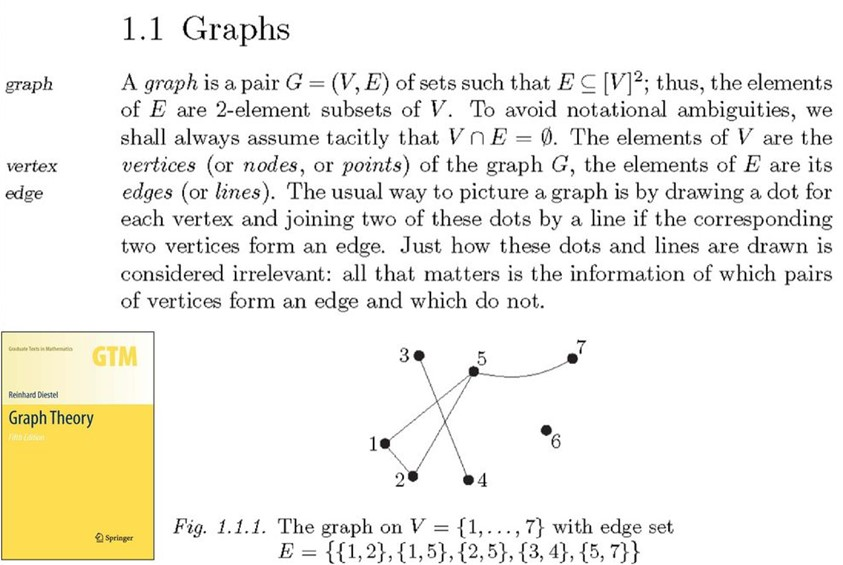
\includegraphics[width=\textwidth]{MathGraphExample.jpg}
    \caption[Voorbeeld wiskundige graaf]{Voorbeeld van een graaf in de wiskunde uit het boek Graph Theory van \textcite{Diestel2010}.}
    \label{mga}
\end{figure}

Graph van Microsoft heeft een soortgelijke betekenis als dat van een wiskundige graaf. Graph staat in voor de verbindingen tussen de entiteiten dat het ondersteunt, in dit geval Microsoft-entiteiten \autocite{Kokkarinen2022}. Een logische interpretatie van Graph wordt weergegeven op Figuur \ref{gms}. \\

\begin{figure}[!b]
    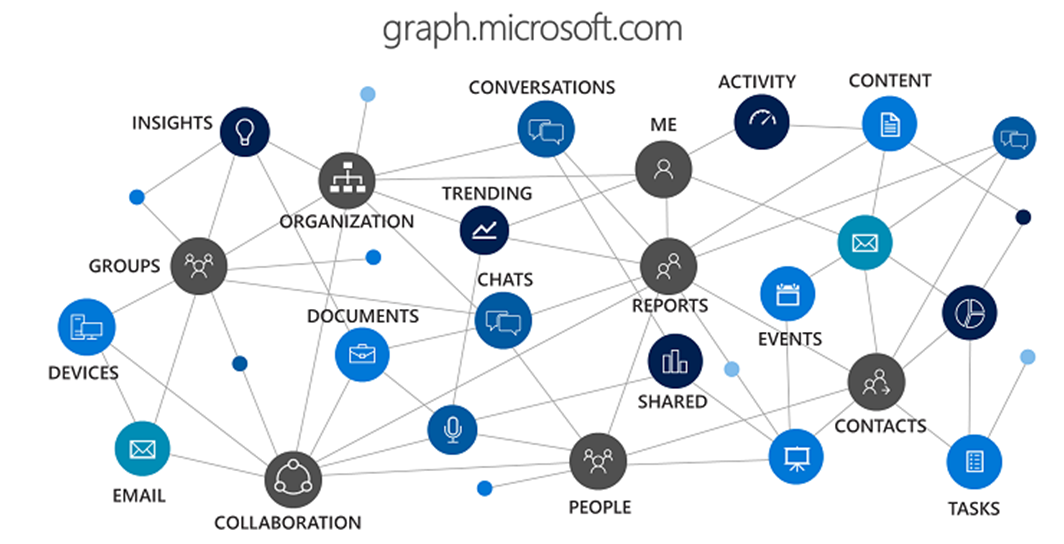
\includegraphics[width=\textwidth]{GraphMicrosoft.png}
    \caption[Voorbeeld Azure AD Graph]{Voorstelling van Azure \Ac{AD} Graph door \textcite{Microsoft2017}.}
    \label{gms}
\end{figure}

\subsubsection{Achterliggende werking van Azure Active Directory Graph API}

% TODO: Bronnen (zie word onder Azure AD Graph API)

% TODO: Schrijf verder vanuit de bron van weareminky, dit is de makkelijkste manier

De Azure \ac{AD} Graph \ac{API} is een OData 3.0-compatibele dienst om objecten zoals gebruikers, groepen en contactpersonen in een tenant te lezen en te wijzigen \autocite{Microsoft2016}. \\

Een tenant kan vergeleken worden met een appartementencomplex \autocite{Saxton2015}. Binnen dit complex zijn meerdere appartementen. In elk appartement heb je bijvoorbeeld een badkamer, slaapkamer, living en balkon. Deze uitleg wordt gevisualiseerd op Figuur \ref{rlt}. \\

\begin{figure}[!h]
    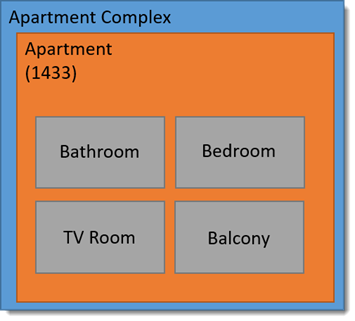
\includegraphics[width=50mm, scale=0.5]{RealTenant.png}
    \caption[Voorbeeld werkelijke tenant]{Voorbeeld van een tenant in het echte leven uit de blog van \textcite{Saxton2015}.}
    \label{rlt}
\end{figure}

In dit scenario met Microsoft is (in \ac{IT}-termen) het complex de Microsoft Office 365-datacenters. Het appartement stelt de tenant of de organisatie in het algemeen voor. Deze tenant-omgeving bevat bijvoorbeeld abonnementen, gebruikers, domeinen en groepen. De tenant wordt gezien als een huurder van de omgeving. Dit concept wordt gevisualiseerd op Figuur \ref{mst}. \\

\begin{figure}[!h]
    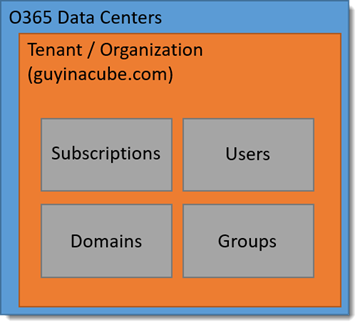
\includegraphics[width=50mm, scale=0.5]{MSTenant.png}
    \caption[Voorbeeld Microsoft tenant]{Voorbeeld van een tenant binnen Microsoft uit de blog van \textcite{Saxton2015}.}
    \label{mst}
\end{figure}

Het OData-protocol dient voor interacties met gegevens via \ac{REST}-webdiensten. Dit protocol biedt een uniforme manier om gegevens en gegevensmodellen te beschrijven \autocite{OData2023}. \\

Door het gebruik van \ac{REST}-eindpunten kunnen \ac{HTTP}-verzoeken verstuurd worden om bewerkingen uit te voeren met de service. De Azure \ac{AD} Graph \ac{API} heeft een eigen demo-omgeving genaamd Azure \ac{AD} Graph Explorer, waarin bepaalde functies en bewerkingen worden getest \autocite{Microsoft}. \\

Het proces van Graph gaat van start wanneer een applicatie een verzoek doet. Dit verzoek moet een token bevatten. Deze token wordt gegeven door Azure \ac{AD} en bewijst dat de gebruiker de juiste machtigingen heeft om de gevraagde data te raadplegen.



\subsubsection{Authenticatie via libraries}

Vooraleer de autorisatie kan plaatsvinden, moet er eerst worden geauthenticeerd. Dit gebeurd via een tool genaamd \ac{ADAL} of de modernere \ac{MSAL} van \textcite{Microsoft2022d}. \\

\ac{ADAL} en \ac{MSAL} worden gebruikt voor verificatie- en autorisatiefunctionaliteiten \autocite{Ooms2022}. Beide technologieën dienen om te kunnen authenticeren met de Graph \ac{API}. \\ 

Er zijn twee methodes om te verbinden met de Graph \ac{API}. \\

De eerste is door middel van een gedelegeerde of interactieve manier. Er wordt gebruikgemaakt van een prompt waarbij de gebruikersnaam (of mailadres) en het wachtwoord wordt gevraagd. \\

Bovendien kan er gevraagd worden om een \ac{2FA}- of \ac{MFA}-methode toe te passen. Dit gaat gepaard met het account waarop de gebruiker wilt inloggen, indien dit geactiveerd is. \\

Het gebruik van \ac{2FA} of \ac{MFA} is veiliger dan alleen het gebruik van een naam en wachtwoord, bevestigt het onderzoek van \textcite{Gunson2011} en \textcite{Banyal2013}. Het wordt sterk aangeraden om minstens \ac{2FA} toe te passen bij het gebruik van een gedelegeerde methode. \\

De tweede methode is door een niet-interactieve of geprogrammeerde manier. Deze methode maakt gebruik van secrets die aan de registratie van een applicatie is gekoppeld. Deze registratie gebeurd in Azure. 



\subsubsection{Autorisatie door middel van tokens}

Azure Active Directory-tokens bevatten informatie over de applicatie, de gebruiker, authenticatie en de rechten die een applicatie mag uitvoeren op de bijhorende directory \autocite{Microsoft2015}. \\

Deze tokens bevinden zich in de autorisatieheader van een verzoek.
Een afgekort voorbeeld hiervan is te zien op Figuur \ref{ahtoken}. \\

\begin{figure}[h]
    \begin{verbatim}Authorization: Bearer eyJ0eX ... FWSXfwtQ
    \end{verbatim}    
    \caption[Voorbeeld Azure AD-token]{Afgekort voorbeeld van een Azure \Ac{AD}-token binnen een autorisatieheader.}
    \label{ahtoken}
\end{figure}

Vervolgens voert de \ac{API} de nodige autorisaties uit via permissie scopes. Dit zijn OAuth 2.0 permissie scopes die aanwezig zijn in het Azure \Ac{AD}-token. OAuth 2.0 is een standaardprotocol voor autorisatie \autocite{OAuth}. \\

De permissie scopes worden gebruikt om te controleren of een gebruiker toegang heeft tot een bepaalde map of locatie. Een ontwikkelaar moet in dit scenario de juiste permissie scopes gebruiken om over de vereiste rechten te beschikken voor een actie. \\

Wanneer er wordt aangemeld, krijgt de gebruiker de mogelijkheid om toestemming te geven of de applicatie in kwestie de mapgegevens van de gebruiker mag benutten. Tijdens het toestaan worden de permissie scopes meegegeven die de ontwikkelaar heeft ingesteld. Een opsomming van de mogelijk permissie scopes binnen de Azure \ac{AD} Graph \ac{API} bevindt zich hieronder. 

\begin{itemize}
    \item User.Read: Rechten om aan te melden en het gebruikersprofiel te lezen.
    \item User.Readbasic.All: Rechten om de basisprofielen van alle gebruikers te lezen.
    \item User.Read.All: Rechten om het volledige profiel van alle gebruikers te lezen.
    \item Group.Read.All: Rechten om alle groepen te lezen.
    \item Group.ReadWrite.All: Rechten om alle groepen te lezen en te bewerken
    \item Device.ReadWrite.All: Rechten om alle apparaten te lezen en te bewerken.
    \item Directory.Read.All: Rechten om alle mapgegevens te lezen.
    \item Directory.ReadWrite.All: Rechten om alle mapgegevens te lezen en te bewerken.
    \item Directory.AccessAsUser.All: Rechten om in de map toe treden als de aangemelde gebruiker.
\end{itemize}

Het gebruik van permissie scopes komt overeen met een gekend veiligheidsprincipe binnen de \ac{IT}. “Principle of Least Privilege”, of “Beginsel van de minste voorrechten” in het Nederlands, staat voor het toekennen van een minimum aan rechten \autocite{Saltzer1975}. 



\subsubsection{Eindpunt adressering}

Om taken of functies uit te voeren met de Graph \ac{API}, wordt er gebruikgemaakt van \ac{HTTP}-verzoeken. Deze verzoeken maken gebruik van een bepaalde methode. Een opsomming van de mogelijk methodes wordt hieronder weergegeven met bijhorende betekenis, gebaseerd op het onderzoek van \textcite{Fielding1999}, \textcite{Dusseault2010}.

\begin{itemize}
    \item GET: Geeft data weer van de server.
    \item POST: Verstuurt data naar de server om nieuwe data aan te maken.
    \item PATCH: Verstuurt data naar de server om gedeeltelijk de bron bij te werken.
    \item PUT: Verstuurt data naar de server om de volledige bron bij te werken.
    \item DELETE: Verwijdert data van de server.
\end{itemize}

Deze verzoeken zijn gericht op een eindpunt van een dienst, rescource, een verzameling of rescource of andere entiteiten die de \ac{API} ondersteunt. De eindpunten worden genoteerd als een \ac{URL}. Het gebruikelijk formaat van zo'n eindpunt wordt voorgesteld op Figuur \ref{bfe}. \\

\begin{figure}[h]
    \footnotesize\begin{verbatim}https://graph.windows.net/{tenant_id}/{resource_path}?{api_version}
    \end{verbatim}    
    \caption[Basis formaat Graph API-eindpunt]{Het basis formaat van een Graph \ac{API}-eindpunt.}
    \label{bfe}
\end{figure}

De reeds voorgestelde \ac{URL} bestaat uit vier componenten.

\begin{itemize}
    \item Service root: Het aanspreekpunt voor alle Graph \ac{API}-verzoeken. Voor Azure \ac{AD} Graph is dit “https://graph.windows.net”.
    \item Tenant Identifier: De identiteit van de tenant waar het verzoek naar gericht is.
    \item Rescource path: Het pad van de bron waar het verzoek naar gericht is.
    \item Graph \ac{API} version: De versie van de \ac{API} waar het verzoek naar gericht is.
\end{itemize}

Een praktisch voorbeeld met betrekking tot het oproepen van gebruikersgegevens, wordt weergegeven op Figuur \ref{pfe}. \\

\begin{figure}[h]
    \footnotesize\begin{verbatim}https://graph.windows.net/contoso.com/users/john@contoso.com/
$links/manager?api-version=1.6
    \end{verbatim}    
    \caption[Voorbeeld Graph API-eindpunt]{Praktisch voorbeeld van een Graph \ac{API}-eindpunt, gericht op de manager eigenschap van “john@contoso.com”.}
    \label{pfe}
\end{figure}



\subsubsection{OData Query Parameters}

Zoals reeds vermeld maar de Graph \ac{API} gebruik van OData. Het gebruik van OData-queryparameters zorgt ervoor dat een ingelezen verzameling van bronnen kunnen gefilterd, gesorteerd en gepagineerd worden. \\

De Graph \ac{API} biedt ondersteuning aan voor de volgende parameters met bijhorende betekenis. De betekenissen staan gedefinieerd in studies van \textcite{Liang2016}, \textcite{Wojcieszyn2014}. 

\begin{itemize}
    \item \$batch: Indienen van \ac{HTTP} POST-verzoeken.
    \item \$expand: Opnemen van een of meerdere bronnen in het antwoord.
    \item \$filter: Filteren van beschikbare bronnen.
    \item \$orderby: Opgeven van ordening door de opgevraagde collectie.
    \item \$previous-page: Ophalen van vorige pagina met resultaten.
    \item \$top: Beperken van een teruggezonden opgevraagde verzameling.
    \item \$skiptoken: Overslaan van opgegeven aantal items.
\end{itemize}

Een toegepast voorbeeld van een OData-queryparameter is te vinden in Figuur \ref{odqp}. \\

\begin{figure}[h]
\footnotesize\begin{verbatim}GET https://graph.windows.net/contoso.com/directoryObjects?api-version=2013-04-05&
$filter=isof('Microsoft.WindowsAzure.ActiveDirectory.User')%20or%20isof
('Microsoft.WindowsAzure.ActiveDirectory.Group')%20or%20isof
('Microsoft.WindowsAzure.ActiveDirectory.Contact')&deltaLink=HTTP/1.1
\end{verbatim}    
\caption[Voorbeeld OData-queryparamter]{Toegepast voorbeeld van een OData-queryparameter op een \ac{HTTP} GET-request.}
\label{odqp}
\end{figure}

\subsubsection{Request en Response Headers}

% TODO: Bron zoeken voor onderstaande uitleg?

De Graph \ac{API} werkt met verzoeken en antwoorden. Een verzoek werkt met een aantal soorten headers en bodies. \\

Drie voorbeelden van voorkomende verzoekheaders zijn de volgende:

\begin{itemize}
    \item Authorization: Uitgegeven Azure \ac{AD}-token.
    \item Content-Type: Mediatype van de inhoud.
    \item Content-Length: Lengte van het verzoek (in bytes).
\end{itemize} 

Daarnaast bestaan er ook een aantal antwoordheaders. Hieronder worden een aantal mogelijke antwoordheaders meegegeven met hun betekenis.

\begin{itemize}
    \item Content-Type: Mediatype van de inhoud.
    \item Location: Antwoord op POST-verzoeken wanneer een nieuwe bron in de directory wordt aangemaakt.
    \item ocp-aad-diagnostics-server-name: Identifier voor de server die een bewerking uitvoert.
    \item ocp-aad-session-key: Sleutel die een sessie met de directorydienst identificeert.
\end{itemize}

Een voorbeeld van antwoordheaders binnen Azure \ac{AD} Graph wordt weergegeven bij Listing \ref{rhaad}. \\

\begin{listing}[h]
\begin{minted}
[
frame=lines,
framesep=2mm,
baselinestretch=1.2,
fontsize=\footnotesize,
linenos
]  
{json}
{
    "cache-control": "no-cache",
    "client-request-id": "140987df-c416-44b8-bf96-16d550256bad",
    "content-length": "12478",
    "content-type": 
        "application/json; 
        odata=minimalmetadata; 
        streaming=true; 
        charset=utf-8",
    "expires": "-1",
    "ocp-aad-session-key": "MzsMU-KCo5fDEUHgzYfj ... hf8ZctaauwL-EZo",
    "pragma": "no-cache",
    "request-id": "c7f02989-6a03-444a-abb2-e3c7993c1ded"
}
    \end{minted}
    \caption[Voorbeeld Response Headers Azure AD Graph]{Voorbeeld van Response Headers binnen Azure \ac{AD} Graph via Azure \Ac{AD} Graph Explorer.}
    \label{rhaad}
\end{listing}

\subsubsection{Request en Response Bodies}

Request bodies kunnen via \Ac{JSON}- of \ac{XML}-payloads verzonden worden voor POST-, PATCH- en PUT-verzoeken. Bovendien kunnen antwoorden (van een server) worden teruggestuurd via \ac{JSON} of \ac{XML}. \\

Het woord “payload” staat voor data die via een pakket of transmissie worden gedragen \autocite{Comer2006}. \\

Deze payloads kunnen in de request bodies gespecifieerd worden via de Content-Type verzoekheader en in antwoorden van Accept-verzoekheaders. \\

Een voorbeeld van een request, met bijhorende request en response body wordt voorgesteld bij Listing \ref{hpr}, \ref{hreqb} en \ref{hresb}. \\

\begin{listing}[h]
\begin{verbatim}
POST https://graph.windows.net/myorganization/users?api-version
\end{verbatim}
\caption[Voorbeeld HTTP POST-request]{Voorbeeld van een \ac{HTTP} POST-request binnen Azure \ac{AD} Graph.}
\label{hpr}
\end{listing}

\begin{listing}[!b]
\begin{minted}
[
frame=lines,
framesep=2mm,
baselinestretch=1.2,
fontsize=\footnotesize,
linenos
]  
{json}
{
    "accountEnabled": true,
    "displayName": "Alex Wu",
    "mailNickname": "AlexW",
    "passwordProfile": {
        "password": "Test1234",
        "forceChangePasswordNextLogin": false
    },
    "userPrincipalName": "Alex@a830edad9050849NDA1.onmicrosoft.com"
}
\end{minted}
\caption[Voorbeeld Request Body Azure AD Graph]{Voorbeeld van een Request Body binnen Azure \ac{AD} Graph.}
\label{hreqb}
\end{listing}

\begin{listing}[!t]
\begin{minted}
[
frame=lines,
framesep=2mm,
baselinestretch=1.2,
fontsize=\footnotesize,
linenos
]  
{json}
{
    "odata.metadata": "https://graph.windows.net/myorganization\n
    /$metadata#directoryObjects/Microsoft.DirectoryServices.User/@Element",
    "odata.type": "Microsoft.DirectoryServices.User",
    "objectType": "User",
    "objectId": "84fba1e8-b942-47c9-a10e-a4bee353ce60",
    "deletionTimestamp": null,
    "accountEnabled": true,
    "assignedLicenses": [],
    "assignedPlans": [],
    "city": null,
    "country": null,
    "department": null,
    "dirSyncEnabled": null,
    "displayName": "Alex Wu",
    "facsimileTelephoneNumber": null,
    "givenName": null,
    "immutableId": null,
    "jobTitle": null,
    "lastDirSyncTime": null,
    "mail": null,
    "mailNickname": "AlexW",
    "mobile": null,
    "onPremisesSecurityIdentifier": null,
    "otherMails": [],
    "passwordPolicies": null,
    "passwordProfile": null,
    "physicalDeliveryOfficeName": null,
    "postalCode": null,
    "preferredLanguage": null,
    "provisionedPlans": [],
    "provisioningErrors": [],
    "proxyAddresses": [],
    "sipProxyAddress": null,
    "state": null,
    "streetAddress": null,
    "surname": null,
    "telephoneNumber": null,
    "usageLocation": null,
    "userPrincipalName": "alex@a830edad9050849NDA1.com",
    "userType": "Member"
}
\end{minted}
\caption[Voorbeeld Response Body Azure AD Graph]{Voorbeeld van een Response Body binnen Azure \ac{AD} Graph.}
\label{hresb}
\end{listing}

\subsection{Toepassingen van Azure AD via PowerShell en Graph} 

% TODO... (Reserve)

Idee: reeds recente voorbeelden illustreren...

Vb. Applicatie voor Teams via de Graph API... 

% ---
% Volgend onderdeel
% ---

\section{Wat is Microsoft Graph?}

Microsoft Graph is, net zoals de reeds besproken Azure \Ac{AD} Graph, een centrale \ac{REST} \ac{API} voor Microsoft-entiteiten. Deze technologie werd door \textcite{Microsoft2015a} in de schijnwerper gezet in 2015. \\

De technologie is gebasseerd op de wiskundige graaf, zoals ook reeds besproken werd bij Azure \Ac{AD} Graph. Microsoft Graph integreert applicaties met verschillende programmeertalen en platformen. Het logisch concept van Graph wordt weergegeven op Figuur \ref{msg}.

\begin{figure}[h]
    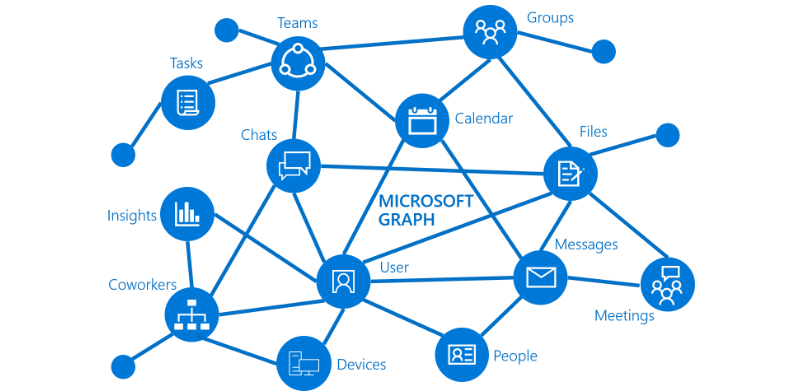
\includegraphics[width=\textwidth]{MicrosoftGraph.png}
    \caption[Voorbeeld Microsoft Graph]{Voorstelling van Microsoft Graph door \textcite{Microsoft2023d}.}
    \label{msg}
\end{figure}

\subsection{Waarom Microsoft Graph als vervanger?}
 
Microsoft Graph is de opvolger van de Azure \ac{AD} PowerShell-modules en bijhorende Azure \Ac{AD} Graph. Op 30 september 2022 maakte Microsoft bekend dat de uitfasering van de Azure \ac{AD} PowerShell-modules en \ac{ADAL} van start zou gaan op 30 juni 2023 \autocite{Sahay2022}. \\

De reden waarom Microsoft deze overgang in gang zet, ontstaat uit volgende redenen volgens \textcite{Microsoft2023e}:

\begin{itemize}
    \item Het gebruik van Microsoft Graph ligt dubbel zo hoog dan dat van Azure \ac{AD} Graph.
    \item Microsoft Graph bevat meer dan 150 nieuwe functies.
    \item Microsoft Graph biedt meer veiligheid en is veerkrachtiger.
    \item Microsoft Graph client libraries bevatten een ingebouwde ondersteuning voor bepaalde functies, waaronder
    \begin{itemize}
        \item herhaalde verwerkingshandelingen,
        \item veilige doorverwijzing,
        \item transparante verificatie,
        \item en payloadcompressie.
    \end{itemize}
    \item Verbeterde mogelijkheden zoals Microsoft 365-groepsbeheer, uitnodiging voor externe gebruikers en anderen.
\end{itemize} 

% TODO Verder schrijven? Navragen!!!

\subsubsection{MSAL als vervanger voor ADAL}

Naast de uitfasering van de Azure \ac{AD} PowerShell-modules, start ook de uitval van \ac{ADAL} op 30 juni 2023. Zoals reeds besproken in Azure \ac{AD} wordt er gebruikgemaakt van \ac{ADAL} of \ac{MSAL} om met de oude als nieuwe Graph te kunnen verbinden. \\

De migratie naar \ac{MSAL} brengt voordelen met zich mee, dat \ac{ADAL} niet kan aanbieden, verklaard \autocite{Microsoft2023m}. Daarnaast is \ac{MSAL} gebouwd om met het Microsoft identity platform te werken, dat de werking met Microsoft Graph vereenvoudigd.



\subsection{Uit wat bestaat Microsoft Graph?}

Microsoft Graph bestaat uit drie toepassingen. \\

De eerste toepassing is de Microsoft Graph \Ac{API}. Dit is een eindpunt dat kan aangesproken worden via “https://graph.microsoft.com” dat Microsoft-entiteiten binnen de cloud kan aanspreken. Dit onderdeel wordt later dieper besproken. \\

De tweede toepassing is Microsoft Graph connectors. Deze Graph-connectoren werken in de ingaande richting. Door het gebruik van deze connectoren, kunnen gegevens buiten de Microsoft-cloud worden gestuurd naar Graph en bijhorende toepassingen. \\

Door het gebruik van deze connectors vermindert de overhead, doordat de informatie bereikbaar is. Deze bereikbaarheid is te danken aan het gebruik van eindpunten zoals SharePoint, Office.com of Bing.com dat de connectors ondersteunen. Op Figuur \ref{MSGC} wordt de werking van Connectors geïllustreerd. \\

\begin{figure}[!h]
    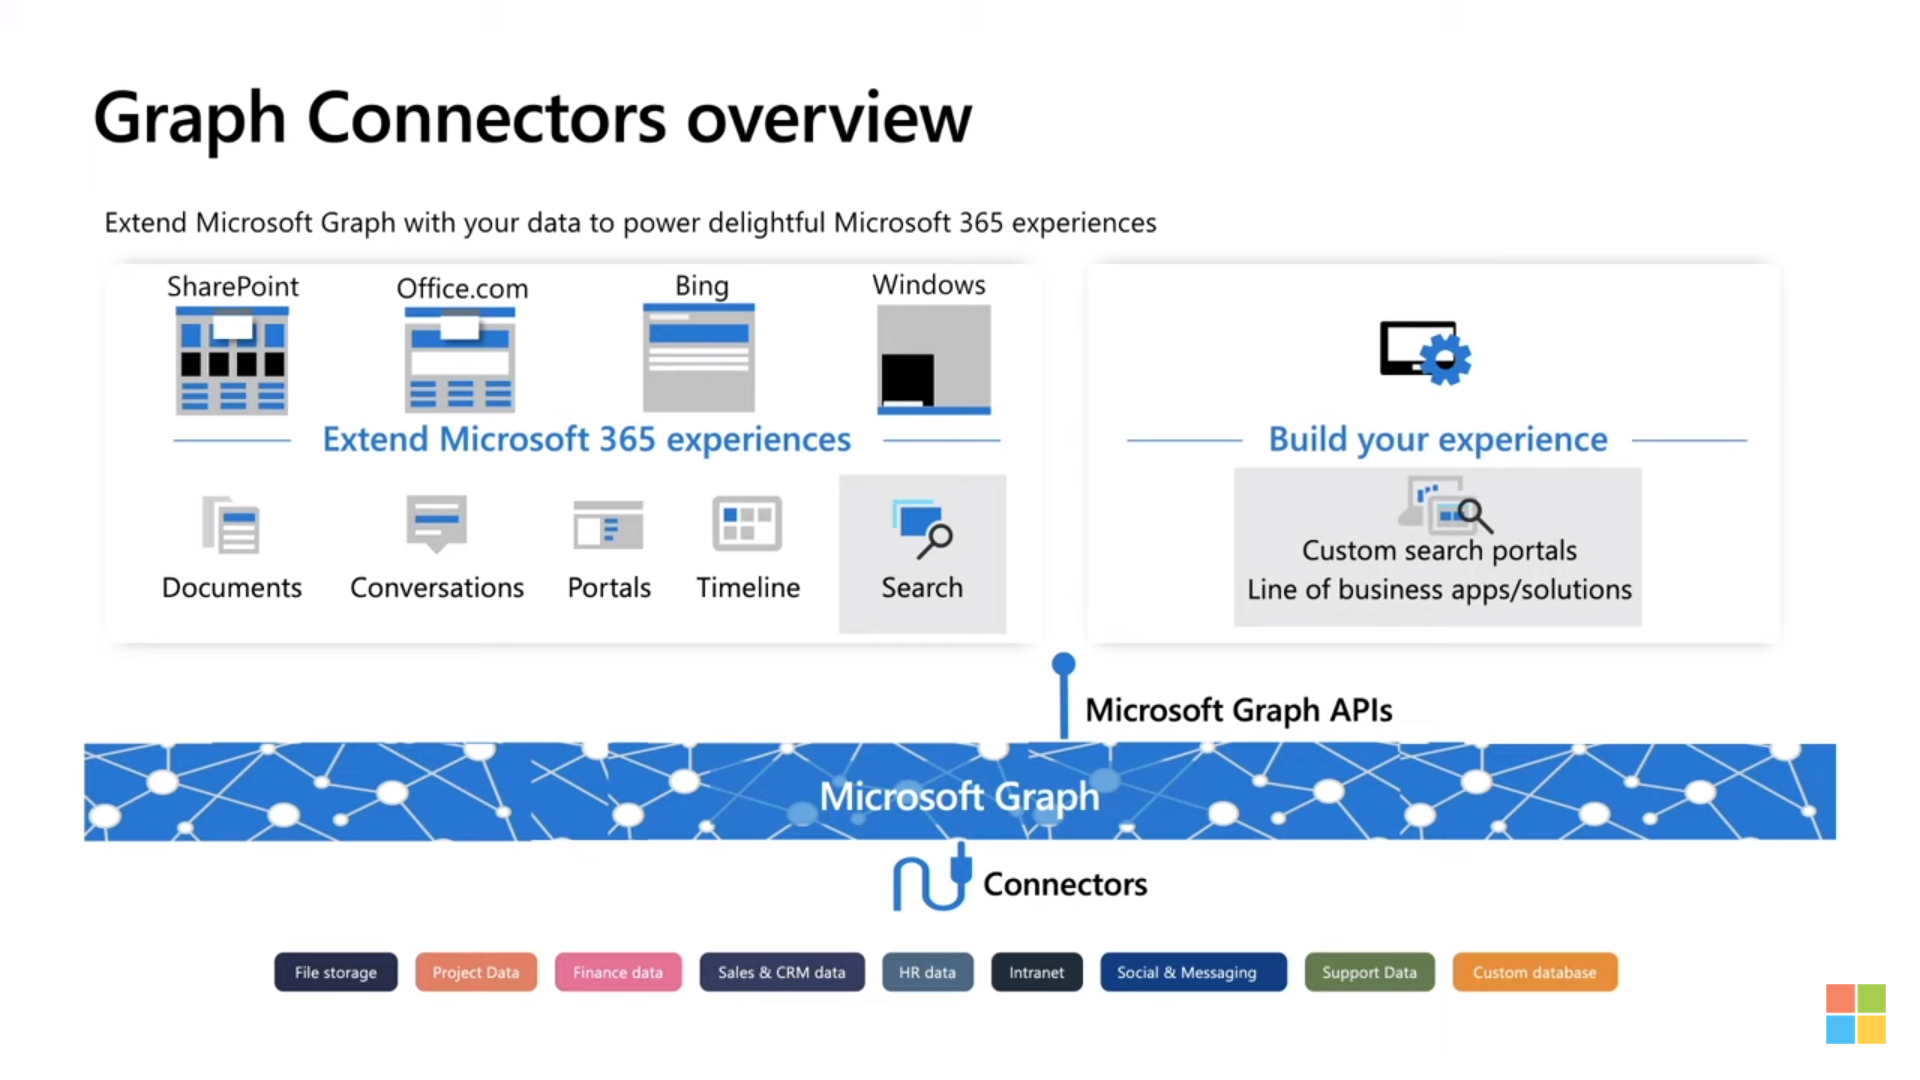
\includegraphics[width=\textwidth]{GraphConnectors.png}
    \caption[Voorbeeld Microsoft Graph Connectors]{Voorstelling van Connectors binnen Microsoft Graph door \textcite{Hay2021}.}
    \label{MSGC}
\end{figure}

Als laatste worden er een set van tools aangeboden via Microsoft Graph Data Connect. Deze tools kunnen gebruikt worden om applicaties te ontwikkelen voor analyse, intelligentie en bedrijfsprocesoptimalisatie met Microsoft 365-data. Deze data wordt geïntegreerd binnen Azure, zodat de reken- en opslagcapaciteiten van het cloudplatform worden gebruikt. Een voorstelling van Data Connect is te zien op Figuur \ref{MSGDC}. \\

\begin{figure}[!h]
    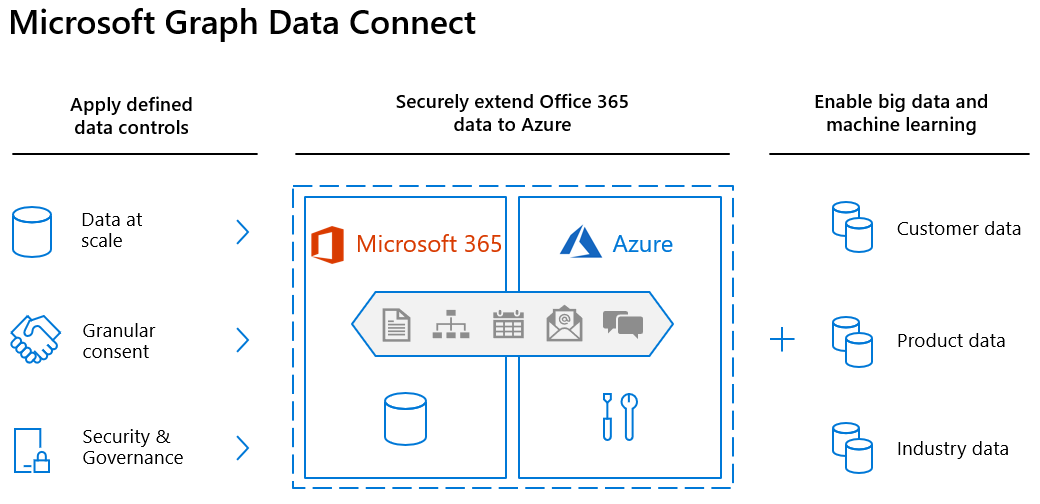
\includegraphics[width=\textwidth]{GraphDataConnect.png}
    \caption[Voorbeeld Microsoft Graph Data Connect]{Voorstelling van Data Connect binnen Microsoft Graph door \textcite{Microsoft2022c}.}
    \label{MSGDC}
\end{figure}

\subsection{Authenticatie en Autorisatie}

Vooraleer er een token wordt uitgegeven, moet een applicatie geregistreerd zijn in het Microsoft identity platform \autocite{Microsoft2022b}. Bovendien moet de applicatie beschikken over de juiste machtigingen om Microsoft Graph te mogen gebruiken. \\

\subsubsection{Toegangsmogelijkheden}

Binnen Microsoft Graph zijn er twee mogelijkheden om toegang te verschaffen tot gegevens. Dit kan via de gedelegeerde- of App-only-methode. Een simpele weergave van wat deze methodes betekenen wordt weergegeven op Figuur \ref{MIPM}. \\

\begin{figure}[h]
    \includegraphics[width=\textwidth]{MIPmethods.png}
    \caption[Voorbeeld toegangsmogelijkheden]{Voorstelling van de twee mogelijke methodes om toegang te krijgen tot het Microsoft identity platform door \autocite{Microsoft2022b}.}
    \label{MIPM}
\end{figure}

De eerste methode, delegated access, staat voor het toegang hebben namens de gebruiker. Dit is mogelijk wanneer een gebruiker zich aanmeldt bij een applicatie. Hierdoor geeft de gebruiker toestemming. Vervolgens kan Microsoft Graph in naam van de gebruiker een actie uitvoeren. Zowel de applicatie als de gebruiker moet over de juiste machtigingen beschikken om het verzoek te laten doorgaan. \\

Een ander woord voor gedelegeerde machtigingen zijn scopes. Deze scopes maken gebruik van OAuth2-permissies. Dit concept werd al reeds besproken bij Azure \ac{AD} Graph. \\

App-only access is de tweede methode. Dit principe werkt zonder een gebruiker om met gegevens te interageren. Dit principe komt eerder voor bij automatische taken (bv. een back-up) of achtergronddiensten (bv. daemons). Dit principe is aan te raden wanneer een gebruiker niet mag inloggen of de vereiste gegevens via meerdere gebruikers worden toegewezen. \\

Bij de tweede methode moet de applicatie over de juiste privileges beschikken. Dit kan via permissies of app-rollen. Een andere manier is via toekennen van eigendomsrechten aan de applicatie. 

\subsubsection{Wat zijn access tokens?}

Access tokens worden verkregen wanneer een toepassing of applicatie een authenticatieverzoek doet. Deze tokens worden gebruikt om de \ac{API} aan te spreken. \\

Als extra veiligheidsprincipe worden toegangstokens van het Microsoft-\newline
identiteitsplatform uitgerust met claims. Claims bevatten extra informatie dat kan dienen als extra validatiemethode. Deze validatie wordt gebruikt om na te kijken of de instantie wel degelijk over de juiste rechten beschikken om bepaalde acties uit te voeren. \\

Deze tokens worden behandeld als ondoorzichtige strings dat alleen voor de \ac{API} bedoeld zijn. Een voorbeeld van een access token is te vinden op Figuur \ref{MSGAT}. \\

\begin{figure}[h]
    \footnotesize\begin{verbatim}eyJ0eXAiOiJKV1QiLCJhb ... lciIUs9DrBLfpCt
\end{verbatim}    
    \caption[Afgekort voorbeeld Microsoft Graph access token]{Afgekort voorbeeld van een access token binnen Microsoft Graph.}
    \label{MSGAT}
\end{figure}

Microsoft Graph wordt aangeroepen door een autorisatieverzoek van een applicatie. De toegangstoken wordt als een Bearer-token gekoppeld aan de Autorisatieheader binnen een \ac{HTTP}-verzoek. Dit concept is gelijkaardig aan dat van een Azure \ac{AD}-token dat al reeds besproken werd. Een voorbeeld van een \ac{HTTP}-verzoek met deze onderdelen wordt weergegeven op Figuur \ref{MSGA}. \\

\begin{figure}[h]
    \footnotesize\begin{verbatim}GET https://graph.microsoft.com/v1.0/me/ HTTP/1.1
Host: graph.microsoft.com
Authorization: Bearer EwAoA8l6BAAU ... 7PqHGsykYj7A0XqHCjbKKgWSkcAg==
    \end{verbatim}    
    \caption[Voorbeeld Microsoft Graph Autorisatieverzoek]{Een voorbeeld van een autorisatieverzoek met een access token binnen Microsoft Graph.}
    \label{MSGA}
\end{figure}

Om aan access tokens te geraken, bestaan er oplossingen zoals authenticatiebibliotheken. Een oplossing van Microsoft is \ac{MSAL} dat voor dit scenario toegankelijk is. Bovendien bestaan er alternatieven zoals Server middleware en authenticatiebibliotheken van derde partijen. \\

Hoe dan ook, deze bibliotheken zijn niet verplicht. Access tokens kunnen ook rechtstreeks verkregen worden als dit gewenst is. 

\subsubsection{Toegang hebben op naam van een gebruiker}

Zoals reeds vermeld, regelen access tokens de toegang tot het gebruik van Microsoft Graph. Om een access token te verkrijgen via een gebruiker, worden de volgende vijf stappen gehanteerd. \\

Als eerste stap moet de applicatie worden geregisteerd bij Azure \ac{AD}. De registratie gebeurd via het onderdeel App Registrations binnen Azure. Wanneer de applicatie geregistreerd is, gaat het Microsoft-identiteitsplatform instaan voor volgende informatie: 

\begin{itemize}
    \item Application ID: Unieke identificatie.
    \item Redirect URI/URL: Eindpunt waar de applicatie wordt op aangesproken.
    \item Client secret: Wachtwoord of sleutelpaar dat gebruikt wordt voor authenticatie. Dit wordt gebruikt bij webapplicaties.
\end{itemize}

Als tweede volgt het autoriseren. Dit gebeurd via het Microsoft identity platform. Via dit platform kan een gebruiker aanmelden en toestemming geven. Bij het verkrijgen van toestemming wordt er een code teruggestuurd. Deze code zorgt voor het verlenen van een access token. Een voorbeeld van deze terugkerende code wordt weergegeven op Figuur \ref{MSGAR}. \\

\begin{figure}[h]
    \footnotesize
    \begin{verbatim}
GET https://localhost/myapp/?
code=M0ab92efe-b6fd-df08-87dc-2c6500a7f84d
&state=12345
    \end{verbatim}    
    \caption[Voorbeeld Microsoft Graph Authorization response]{Een voorbeeld van een autorisatie antwoord met de nodige code om een access token te verkrijgen binnen Microsoft Graph.}
    \label{MSGAR}
\end{figure}

Daarna moet er een token worden verkregen. Dit gebeurd via een tokenverzoek dat op Figuur \ref{HTR} wordt weergegeven. Na het versturen van dit verzoek volgt er een antwoord met een access token in \ac{JSON}-formaat. Dit antwoord wordt voorgesteld op Figuur \ref{HTRES}. \\ 

\begin{figure}[!h]
    \footnotesize\begin{verbatim}
POST /common/oauth2/v2.0/token HTTP/1.1
Host: https://login.microsoftonline.com
Content-Type: application/x-www-form-urlencoded
        
client_id=6731de76-14a6-49ae-97bc-6eba6914391e
&scope=user.read%20mail.read
&code=OAAABAAAAiL9Kn2Z27UubvWFPbm0gLWQJVzCTE9UkP3pSx1aXxUjq3n8b2JRLk4OxVXr...
&redirect_uri=http%3A%2F%2Flocalhost%2Fmyapp%2F
&grant_type=authorization_code
&client_secret=JqQX2PNo9bpM0uEihUPzyrh
    \end{verbatim}    
    \caption[Voorbeeld User Token Request Microsoft Graph]{Een voorbeeld van een tokenverzoek via \ac{HTTP} binnen Microsoft Graph.}
    \label{HTR}
\end{figure}

\begin{figure}[!h]
    \footnotesize\begin{verbatim}
{
    "token_type": "Bearer",
    "scope": "user.read%20Fmail.read",
    "expires_in": 3600,
    "access_token": "eyJ0eXAiOiJKV1QiLCJhbGciOiJSUzI1NiIsIng1dCQ...",
    "refresh_token": "AwABAAAAvPM1KaPlrEqdFSBzjqfTGAMxZGUTdM0t4B4..."
}        
    \end{verbatim}    
    \caption[Voorbeeld User Token Response Microsoft Graph]{Een voorbeeld van een tokenantwoord via \ac{JSON} binnen Microsoft Graph.}
    \label{HTRES}
\end{figure}

Vervolgens wordt de verkregen token gebruikt om Microsoft Graph op te roepen. Het toegankstoken wordt in de autorisatieheader van een verzoek geplaatst. Dit werd al reeds voorgesteld op Figuur \ref{MSGA}. \\

Als laatste volgt het gebruik van een refresh token. Een refresh token ververst de duur van een toegangstoken, doordat een toegangstoken kan vervallen. Een verzoek en antwoord, met het gebruik van refresh tokens, is te vinden op Figuur \ref{MSGRTR} en \ref{MSGRTRES}.

\begin{figure}[!h]
    \footnotesize\begin{verbatim}
POST /{tenant}/oauth2/v2.0/token HTTP/1.1
Host: https://login.microsoftonline.com
Content-Type: application/x-www-form-urlencoded

client_id=11111111-1111-1111-1111-111111111111
&scope=user.read%20mail.read
&refresh_token=OAAABAAAAiL9Kn2Z27UubvWFPbm0gLWQJVzCTE9UkP3pSx1aXxUjq...
&grant_type=refresh_token
&client_secret=jXoM3iz...   
    \end{verbatim}    
    \caption[Voorbeeld Refresh Token request Microsoft Graph]{Een voorbeeld van een verzoek met een refresh token via \ac{HTTP} binnen Microsoft Graph.}
    \label{MSGRTR}
\end{figure}

\begin{figure}[!h]
    \footnotesize\begin{verbatim}
{
    "access_token": "eyJ0eXAiOiJKV1QiLCJhbGciOiJSUzI1NiIsIng1dCI6Ik5HVEZ2ZEstZnl0aEV1Q...",
    "token_type": "Bearer",
    "expires_in": 3599,
    "scope": "user.read%20mail.read",
    "refresh_token": "AwABAAAAvPM1KaPlrEqdFSBzjqfTGAMxZGUTdM0t4B4...",
}    
    \end{verbatim}    
    \caption[Voorbeeld Refresh Token response Microsoft Graph]{Een voorbeeld van een antwoord met een refresh token via \ac{JSON} binnen Microsoft Graph.}
    \label{MSGRTRES}
\end{figure}

\subsubsection{Toegang hebben zonder een gebruiker}

De tweede manier om een access token te verkrijgen, is zonder het gebruik van een user. Dit zijn de volgende vijf stappen gehanteerd. \\

De eerste stap is het registreren van een applicatie. Dit komt overeen met de uitleg die in de eerste manier werd beschreven. \\

Vervolgens moeten de permissies van Microsoft Graph worden geconfigureerd. Dit is nodig zodat een applicatie zonder toestemming een token mag aanvragen. Dit kan geconfigureerd worden onder “Request \ac{API} permission” bij het registratieportaal voor applicaties binnen Azure. \\

De derde stap omvat het verkrijgen van toegang door de beheerder. Het verkijgen van toegang door een beheerder kan gebeuren op twee manieren. De eerste manier is via Azure, door het gebruik van het portaal. De andere optie is via het Microsoft identity platform door middel van een verzoek naar het adminconsent-eindpunt. Een bijhorend voorbeeld van een verzoek en antwoord wordt weergegeven op \ref{MSGRAR} en \ref{MSGRARES}. \\

\begin{figure}[!h]
    \footnotesize\begin{verbatim}
GET https://login.microsoftonline.com/{tenant}/adminconsent
?client_id=6731de76-14a6-49ae-97bc-6eba6914391e
&state=12345
&redirect_uri=https://localhost/myapp/permissions
    \end{verbatim}    
    \caption[Voorbeeld Adminconsent request Microsoft Graph]{Een voorbeeld van een verzoek voor toestemming van de beheerder via \ac{HTTP} binnen Microsoft Graph.}
    \label{MSGRAR}
\end{figure}

\begin{figure}[!h]
    \footnotesize\begin{verbatim}
GET https://localhost/myapp/permissions
?tenant=a8990e1f-ff32-408a-9f8e-78d3b9139b95&state=12345
&admin_consent=True
    \end{verbatim}    
    \caption[Voorbeeld Adminconsent respons Microsoft Graph]{Een voorbeeld van een antwoord voor toestemming van de beheerder via \ac{HTTP} binnen Microsoft Graph.}
    \label{MSGRARES}
\end{figure}

Bij de vierde stap moet er een access token aanwezig zijn. Dit principe komt overeen met de derde stap van de vorige methode. Een voorbeeld van een verzoek en antwoord binnen deze stap wordt weergegeven op Figuur \ref{MSGATRR} en \ref{MSGATRRES}. \\

\begin{figure}[!h]
    \footnotesize\begin{verbatim}
POST https://login.microsoftonline.com/{tenant}/oauth2/v2.0/token HTTP/1.1
Host: login.microsoftonline.com
Content-Type: application/x-www-form-urlencoded

client_id=535fb089-9ff3-47b6-9bfb-4f1264799865
&scope=https%3A%2F%2Fgraph.microsoft.com%2F.default
&client_secret=qWgdYAmab0YSkuL1qKv5bPX
&grant_type=client_credentials 
    \end{verbatim}    
    \caption[Voorbeeld Application Token Request Microsoft Graph]{Een voorbeeld van een verzoek met een applicatie access token via \ac{HTTP} binnen Microsoft Graph.}
    \label{MSGATRR}
\end{figure}

\begin{figure}[!h]
    \footnotesize\begin{verbatim}
{
    "token_type": "Bearer",
    "expires_in": 3599,
    "ext_expires_in":3599,
    "access_token": "eyJ0eXAiOiJKV1QiLCJhbGciOiJSUzI1NiIsIng1dCI6Ik1uQ19WWmNBVGZNNXBP..."
} 
    \end{verbatim}    
    \caption[Voorbeeld Application Token Response Microsoft Graph]{Een voorbeeld van een antwoord met een applicatie access token via \ac{JSON} binnen Microsoft Graph.}
    \label{MSGATRRES}
\end{figure}

De vijfde stap is het gebruiken van de access token om Microsoft Graph op te roepen. Dit komt overeen met de vierde stap van de eerste manier. Er wordt een verzoek gedaan met een access token dat verkregen werd. Een voorbeeld van dit verzoek is te vinden op Figuur \ref{MSGAAT}.

\begin{figure}[!h]
    \footnotesize\begin{verbatim}
GET https://graph.microsoft.com/v1.0/users/12345678-73a6-4952-a53a-e9916737ff7f
Authorization: Bearer eyJ0eXAiO ... 0X2tnSQLEANnSPHY0gKcgw
Host: graph.microsoft.com
    \end{verbatim}    
    \caption[Voorbeeld Application autorisatieverzoek Microsoft Graph]{Een voorbeeld van een autorisatieverzoek met een application access token via \ac{HTTP} binnen Microsoft Graph.}
    \label{MSGAAT}
\end{figure}



\subsection{Microsoft Graph API}

Zoals vermeld is de Microsoft Graph \Ac{API} gebasseerd op \Ac{REST}. Door het gebruik van de \ac{API} zijn de cloud-servicebronnen van Microsoft beschikbaar. \\

Om tot deze bronnen toegang te hebben en om de \Ac{API} aan te spreken, moeten er twee acties voldaan zijn:

\begin{itemize}
    \item De applicatie is geregistreerd.
    \item Er zijn authenticatietokens verkregen voor een gebruiker of instantie.
\end{itemize}

\subsubsection{OData}

De \ac{API} maakt gebruik van OData. OData werd al reeds besproken in het vorige onderdeel, dit wordt dus niet nog eens aangekaart. Door het gebruik van OData kunnen bronnen, methodes en opsommingen in de metadata van Microsoft Graph worden gedefinieerd.

\subsubsection{REST API}

Om naar een bron te schrijven of te lezen, wordt er gebruikgemaakt van een verzoek. De opbouw van een verzoek wordt weergegeven op Figuur \ref{RAM}. \\

\begin{figure}[h]
    \footnotesize\begin{verbatim}{HTTP method} https://graph.microsoft.com/{version}/{resource}?{query-parameters}
    \end{verbatim}    
    \caption[Basis formaat Microsoft Graph API-eindpunt]{Het basis formaat van een Microsoft Graph \Ac{API}-eindpunt.}
    \label{RAM}
\end{figure}

Een verzoek bestaat uit vier componenten, namelijk het volgende:

\begin{itemize}
    \item \ac{HTTP} method: Een \ac{HTTP}-methode dat gebruik wordt voor het verzoek.
    \item version: De versie van de \ac{API} dat de bijhorende applicatie ondersteunt.
    \item rescource: De bron of rescource dat gebruikt wordt.
    \item query-parameters: Optionele OData-queryparameters of \Ac{REST}-methodes dat het antwoord aanpassen.
\end{itemize}

% TODO: nakijken!
\begin{comment}
Wanneer er een verzoek wordt verstuurd, krijgt dit ook een antwoord terug. Een antwoord bestaat uit minstens volgende onderdelen: 

\begin{itemize}
    \item Status code:
    \item Response message:
    \item @odata.nextLink:
\end{itemize}
\end{comment}

\subsubsection{HTTP methods}

Microsoft Graph werkt met \Ac{HTTP}-methodes bij een verzoek. Microsoft Graph maakt gebruik van vijf soorten methodes, namelijk:

\begin{itemize}
    \item GET
    \item POST
    \item PATCH
    \item PUT
    \item DELETE
\end{itemize}

De betekenis van deze vijf methodes werd al reeds aangehaald bij Azure \Ac{AD} Graph. \\

De GET- en DELETE-methode vallen onder CRUD-methodes. CRUD staat voor CREATE, READ, UPDATE en DELETE \autocite{Truica2015}. De CRUD-operaties komen voor in het \ac{IT}-component rond databanken. In Microsoft Graph staan GET en DELETE gelijk aan de CRUD-operaties READ en DELETE. Bovendien maken deze twee methodes geen gebruik van een request body. \\

De andere drie methodes (POST, PATCH en PUT) gebruiken wel een request body. Meestal wordt in dit deel van het verzoek gebruikgemaakt van het \ac{JSON}-formaat. In dit formaat wordt er extra informatie meegeven over welke waarden moeten gebruikt worden voor een operatie of methode uit te voeren. Een voorbeeld van een request met bijhorend antwoord is te vinden op Figuur \ref{MSPR} en \ref{MSPRES}. \\

\begin{figure}[h]
    \footnotesize\begin{verbatim}POST
https://graph.microsoft.com/v1.0/tenantRelationships/delegatedAdminRelationships/
5d027261- ... -a3205431b836/requests
Content-Type: application/json

{
    "action": "lockForApproval"
}
    \end{verbatim}    
    \caption[Voorbeeld Microsoft Graph POST-verzoek]{Een voorbeeld van een \ac{HTTP} POST-verzoek binnen Microsoft Graph.}
    \label{MSPR}
\end{figure}

\begin{figure}[h]
    \footnotesize\begin{verbatim}
HTTP/1.1 201 Created
Content-Type: application/json
Location: https://graph.microsoft.com/v1.0/tenantRelationships/
delegatedAdminRelationships/c45e5ffb- ... -25a5a3fbf339

{
    "@odata.type": "#microsoft.graph.delegatedAdminRelationshipRequest",
    "@odata.context": "https://graph.microsoft.com/v1.0\n
    /tenantRelationships/$metadata#requests",
    "id": "5a6666c9-7282-0a41-67aa-25a5a3fbf339",
    "action": "lockForApproval",
    "status": "created",
    "createdDateTime": "2022-02-10T10:55:47.1180588Z",
    "lastModifiedDateTime": "2022-02-10T10:55:47.1180588Z"
}
    \end{verbatim}    
    \caption[Voorbeeld Microsoft Graph POST-antwoord]{Een voorbeeld van een \ac{HTTP} POST-antwoord binnen Microsoft Graph.}
    \label{MSPRES}
\end{figure}

\subsubsection{Beschikbare versies}

Microsoft Graph is volop in ontwikkeling en ondersteunt, op dit moment van het schrijven, twee versies \Autocite{Microsoft2023f}. \\

De eerste versie, onder de naam v1.0, is een stabiele versie dat toegepast kan worden in productieomgevingen en -applicaties. \\

De tweede versie, onder de naam beta, is een versie waar actief aan (nieuwe) concepten gesleuteld wordt. Deze versie wordt toegepast in testomgevingen, doordat het nog in ontwikkeling is. Het wordt niet aangeraden voor in productie te gebruiken. 

\subsubsection{Wat zijn resources?}

Bronnen, of beter bekend als rescources, zijn entiteiten of types die gebruikt worden om de communicatie met een verzoek mogelijk te maken. Zoals in de \ac{URL} weergegeven, komt een rescource hierin voor. \\

Mogelijke bronnen zijn bijvoorbeeld “me”, een user, een groep, etc. Deze bronnen ondersteunen ook relaties, waardoor andere onderdelen aangesproken kunnen worden. Ter illustratie, wanneer er een gebruiker een mail wilt sturen, is dit mogelijk via “me/sendMail”. Een voorbeeld van het gebruik van een resource is te vinden op Figuur \ref{MSGR}. \\

\begin{figure}[h]
    \footnotesize\begin{verbatim}GET https://graph.microsoft.com/v1.0/me/onenote/resources/{id}/content
    \end{verbatim}    
    \caption[Voorbeeld Microsoft Graph resource]{Een voorbeeld van een “me/onenote” resource binnen Microsoft Graph.}
    \label{MSGR}
\end{figure}

Bronnen vereisen machtigingen om bepaalde acties uit te voeren. Hier moet rekening mee gehouden worden voor er een actie wordt uitgevoerd.

\subsubsection{Responses aanpassen via queryparameters}

Antwoorden of responses worden weergegeven na het gebruik van een bepaald HTTP-verzoek. Het antwoord kan aangepast worden via twee soorten queryparameters. \\

Als eerste de OData-queryparameters. Deze queryparamaters zijn afkomstig van het OData-protocol waarvan bepaalde parameters worden ondersteund door \textcite{Microsoft2023g}. Een toegepast voorbeeld van een verzoek met een OData-queryparameter wordt weergegeven op Figuur \ref{TRAM}. \\

\begin{figure}[h]
    \footnotesize\begin{verbatim}GET https://graph.microsoft.com/v1.0/me?$select=displayName,jobTitle
    \end{verbatim}    
    \caption[Voorbeeld OData HTTP-verzoek]{Praktisch OData voorbeeld van een Microsoft Graph \Ac{API}-eindpunt, waarbij er op “displayName” en “jobTitle” wordt gefilterd.}
    \label{TRAM}
\end{figure}

Het tweede soort dat antwoorden kan aanpassen zijn de normale queryparameters. Met het woord normaal worden niet-OData-gerelateerde parameters bedoelt. Een voorbeeld van dit soort queryparameters is te vinden op Figuur \ref{NRAM}. \\

\begin{figure}[h]
    \footnotesize\begin{verbatim}GET https://graph.microsoft.com/me/calendarView?startDateTime=
2019-09-01T09:00:00.0000000&endDateTime=2019-09-01T17:00:00.0000000
    \end{verbatim}    
    \caption[Voorbeeld niet-OData HTTP-verzoek]{Praktisch niet-OData voorbeeld van een Microsoft Graph \Ac{API}-eindpunt, waarbij een bepaalde tijdsperiode wordt opgevraagd.}
    \label{NRAM}
\end{figure}

\subsubsection{Tools om de Microsoft Graph API te testen}

De werking van Microsoft Graph API kan worden getest in een demo-omgeving. Deze omgeving wordt Graph Explorer genoemd en wordt voorzien door \textcite{Microsoft2023h}. Hierin kunnen verzoeken worden getest met of zonder Microsoft-tenant. \\

Daarnaast kan de API ook worden getest via Postman. Postman is een collaboratief \ac{API}-platform dat los van Microsoft staat \autocite{Postman2023}.

% TODO: \subsubsection{MSAL ...}

\subsection{Microsoft Graph met PowerShell}

Microsoft Graph kan worden aangestuurd met PowerShell \autocite{Microsoft2023j}. Deze PowerShell-integratie zit in de Microsoft Graph PowerShell \ac{SDK}. Een \ac{SDK} bestaat uit een verzameling van tools dat instaan voor het maken van bepaalde software of hardware \autocite{RedHat2020}. Deze PowerShell \ac{SDK} stelt de \ac{API} van Microsoft Graph bloot. Door deze blootstelling kan PowerShell de \ac{API} gebruiken, beheren en automatiseren.

\subsubsection{Ondersteunende dependencies}

Microsoft Graph PowerShell ondersteunt een lijst van dependencies \autocite{Microsoft2023k}. Een overzicht van alle ondersteunde dependencies is te vinden in Tabel \ref{MSGDT}. 

\begin{table}
    \small
    \centering
    \begin{tabular}{ |c| } 
        \hline
        \textbf{Dependencies (tot aan versie 1.23)} \\
        \hline
        Applications \\
        Authentication \\
        Bookings \\
        Calender \\
        Changing Notifications \\
        Cloud Communications \\
        Compliance \\
        Cross Device Experiences \\
        Device Management \\
        Device Management Actions \\
        Device Management Administration \\
        Device Management Enrolment \\
        Device Management Functions \\
        Devices Cloud Print \\
        Devices Corporate Management \\
        Devices Service Announcement
        Directory Objects \\
        Education \\
        Files \\
        Financials \\
        Groups \\
        Identity Directory Management \\
        Identity Governance \\
        Identity Sign-ins \\
        Mail \\
        Managed Tenants \\
        Notes \\
        People \\
        Personal Contacts \\
        Planner \\
        Reports \\
        Schema Extensions \\
        Search \\
        Sites \\
        Teams \\
        Users \\
        Users Actions \\
        Users Funtions \\
        Windows Updates \\
        \hline
    \end{tabular}
    \caption[Tabel Microsoft Graph dependencies]{Tabel met overzicht van alle ondersteunende dependencies tot aan versie 1.23 binnen Microsoft Graph PowerShell.}
    \label{MSGDT}
\end{table}

\subsubsection{Geïntegreerde data-objecten van Azure AD}

Door de uitfasering van Azure \ac{AD} PowerShell, worden de data-objecten van de AzureAD-module geïntegreerd binnen Microsoft Graph \autocite{Microsoft2023l}. Een overzicht van deze integratie wordt weergegeven in Tabel \ref{MSGDOT}.

\begin{table}
    \small
    \centering
    \begin{tabular}{ |c|c| } 
        \hline
        \textbf{Geïntegreerd data-object} & \textbf{Aantal commando's} \\
        \hline
        Administrative Units & 9 \\ 
        Applications & 20 \\ 
        AzureAD & 48 \\ 
        Certificate Authorities & 1 \\ 
        Connect to directory & 2 \\ 
        Contacts & 7 \\ 
        Contracts & 1 \\ 
        Deleted Objects & 1 \\ 
        Devices & 9 \\    
        Directory & 3 \\
        Directory Objects & 1 \\ 
        Directory Roles & 13 \\ 
        Domains & 8 \\ 
        Extension Properties & 1 \\ 
        Groups & 26 \\ 
        OAuth2 & 2 \\ 
        Policies & 2 \\ 
        Service Principals & 22 \\ 
        Users & 30 \\ 
        \hline
    \end{tabular}
    \caption[Tabel geïntegreerde data-objecten]{Tabel met overzicht van alle geïntegreerde data-objecten met bijhorende commando's binnen Microsoft Graph PowerShell.}
    \label{MSGDOT}
\end{table}

\subsection{Toepassingen van Microsoft Graph}

% TODO ...
%%=============================================================================
%% Methodologie
%%=============================================================================

\chapter{\IfLanguageName{dutch}{Methodologie}{Methodology}}%
\label{ch:methodologie}

%% TODO: Hoe ben je te werk gegaan? Verdeel je onderzoek in grote fasen, en
%% licht in elke fase toe welke stappen je gevolgd hebt. Verantwoord waarom je
%% op deze manier te werk gegaan bent. Je moet kunnen aantonen dat je de best
%% mogelijke manier toegepast hebt om een antwoord te vinden op de
%% onderzoeksvraag.

Om een antwoord te vinden op deze onderzoeksvraag, worden de volgende stappen gehanteerd. \\

Als eerste wordt het onderzoeksdomein volledig gekaderd aan de hand van een literaire stand van zaken. Na het verzamelen en verwerken van alle literaire studies, volgt de vergelijking tussen het oude en het nieuwe. Zoals reeds vermeld wordt de PowerShell-module en \ac{API} van Azure \ac{AD} uitgefaseerd. Azure \ac{AD} wordt gezien als het “oude”. De nieuwe Microsoft Graph, de vervanger van Azure \ac{AD}, wordt gezien in de vergelijking als het “nieuwe”. \\

De vergelijking tussen de twee bevat de eerste helft van het antwoord op de onderzoeksvraag. In deze vergelijking wordt er gekeken naar vier onderdelen of criteria's. 

\begin{itemize}
    \item Werking van de \ac{API}: Wat zijn de mogelijke \Ac{HTTP}-verzoeken? Uit welke onderdelen bestaat het eindpunt? Zijn er verschillen aanwezig in requests en reponses tijdens het uitvoeren van een query? Welke PowerShell-versies zijn er?
    \item Aanspreekbare data-objecten en dependencies: Welke data-objecten kunnen worden aangesproken? Bevat de technologie bepaalde afhankelijkheden?
    \item Toegangsmogelijkheden: Hoe wordt er toegang verschaft tot de technologie? 
    \item Security: Zijn de toegangsmogelijkheden veilig? Wordt er gebruikgemaakt van rechten om misbruik tegen te gaan?
\end{itemize}

Met deze vier onderdelen wordt de vergelijking tussen het oude en het nieuwe uitgevoerd. Deze vergelijking wordt aan de hand van de verwerkte literatuur toegepast. \\

Om de tweede helft van het antwoord te geven op de onderzoeksvraag wordt de casus praktisch uitgewerkt in een Proof-of-Concept. Het verouderde auditing-script van Easi, dat geschreven is in PowerShell, maakt gebruik van de verouderde modules. Dit script wordt vernieuwd door middel van de modernere Microsoft Graph PowerShell-modules. Door dit script te herwerken wordt er op een praktisch manier aangetoond wat vandaag de dag wel en niet mogelijk is met Microsoft Graph. \\

Tijdens de uitwerking van de Proof-of-Concept wordt er gewerkt met een vijf-stappenplan. Als eerste, het bekijken en beschrijven van de startende data-set na het activeren van de licentie. Als tweede, de data-set aanpassen naar een nagebootste klantenomgeving. Deze nabootsing wordt op basis van een intern document binnen Easi uitgevoerd. Daarna, het aanmaken van een Microsoft Graph-applicatie. Vervolgens, het maken van een PowerShell-script om de testomgeving aan te spreken. Als laatste, het omvormen van het verouderde PowerShell-script dat Easi gebruikt.

Om dit script zo efficiënt mogelijk te herwerken, worden twintig kleinere onderdelen van dit script behandeld. Deze twintig onderdelen of functies maken gebruik van de uitfaserende Azure \ac{AD} PowerShell-module. Hieronder worden de twintig functies opgesomd met een korte beschrijving. 

\begin{enumerate}
    \item Aantal aanwezige domeinen binnen de Office 365-omgeving.
    \item Aantal gebruikers binnen de omgeving, onderverdeeld in interne
    en extene gebruikers.
    \item Aantal gebruikers die geblokkeerd zijn.
    \item Aantal geblokkeerde gebruikers met actieve licenties.
    \item Overzicht en telling van administrators met hun account status.
    \item Overzicht en telling van de interne gebruikers met \ac{MFA}.
    \item Aantal gelicenseerde, actieve accounts waarbij \ac{MFA} niet aanwezig is.
    \item Aantal externe accounts waarbij \ac{MFA} uitstaat.
    \item Overzicht van accounts met administrator-priviliges,
    onderverdeeld in gebruik van \ac{MFA}.
    \item Groottes van elk type mailbox.
    \item Groottes van elke mailbox, gerangschikt van groot naar klein.
    \item Onderverdeling van gebruikersmailboxen op basis van grootte.
    \item Onderverdeling van gedeelde mailboxen op basis van grootte.
    \item Onderverdeling van hoeveelheid mailboxen per domein.
    \item Overzicht van accounts met als primair \Ac{SMTP}-adresdomein “.onmicrosoft.com”.
    \item Overzicht gedeelde mailboxen, onderverdeeld in aanwezigheid van een licentie.
    \item Overzicht van verborgen mailboxen.
    \item Overzicht van \ac{SMTP}-forwarding.
    \item Overzicht verschillende types van licenties en het aantal personen met dit licentietype.
    \item Overzicht verschillende methodes waarop \ac{MFA} wordt gebruikt met hoeveelheid gebruikers, onderverdeeld op basis van methode.
\end{enumerate}

Binnen deze twintig onderdelen zijn er vijf groepen van data. Dit zijn de vijf soorten data dat worden nagekeken wanneer klanten een audit uitvoeren door Easi. De vijf groepen worden hieronder weergegeven. 

\begin{itemize}
    \item Domeinen
    \item Gebruikers
    \item Licenties
    \item Mailboxen
    \item \ac{MFA}
\end{itemize}

Tijdens de praktische uitwerking wordt er gebruikgemaakt van de Microsoft Graph PowerShell-modules. In het specifiek, de meest recente versie van de eerste stabiele uitrol dat beschikbaar is tijdens de uitvoering van dit onderzoek, namelijk versie 1.25 \autocite{Microsoft2023k}. De mogelijkheid is reëel dat er tijdens of na de uitwerking een recentere versie zal worden uitgegeven door Microsoft. Er wordt niet afgeweken van versie 1.25 met bijhorende modules in dit onderzoek. \\  

Wanneer het onderdeel kan worden uitgevoerd via de PowerShell-modules van Microsoft Graph, dan wordt er een PowerShell-script uitgewerkt voor dat onderdeel. Dit bewijst dat Microsoft Graph kan gebruikt worden voor de vervanging van Azure \ac{AD} en MSonline van het audit-script. \\

Als een onderdeel niet kan worden uitgevoerd via de Microsoft Graph PowerShell-modules, dan wordt er dieper gekeken naar het bijhorende domein. Er wordt uitgezocht dat het domein wel of niet ondersteund wordt door de PowerShell-modules van Microsoft Graph. Een mogelijk alternatief wordt besproken, maar de uitwerking hiervan valt buiten de scope van dit onderzoek. \\

Uiteindelijk wordt een conclusie gevormd op basis van beide helften uit dit onderzoek. 

% === END ====

% Voeg hier je eigen hoofdstukken toe die de ``corpus'' van je bachelorproef
% vormen. De structuur en titels hangen af van je eigen onderzoek. Je kan bv.
% elke fase in je onderzoek in een apart hoofdstuk bespreken.

%\input{...}
%\input{...}
%...

%%=============================================================================
%% Conclusie
%%=============================================================================

\chapter{Conclusie}%
\label{ch:conclusie}

% TODO: Trek een duidelijke conclusie, in de vorm van een antwoord op de
% onderzoeksvra(a)g(en). Wat was jouw bijdrage aan het onderzoeksdomein en
% hoe biedt dit meerwaarde aan het vakgebied/doelgroep? 
% Reflecteer kritisch over het resultaat. In Engelse teksten wordt deze sectie
% ``Discussion'' genoemd. Had je deze uitkomst verwacht? Zijn er zaken die nog
% niet duidelijk zijn?
% Heeft het onderzoek geleid tot nieuwe vragen die uitnodigen tot verder 
%onderzoek?

% taal ok

In dit onderzoek wordt er een antwoord gegeven op de onderzoeksvraag: “Is Microsoft Graph klaar om de beheertaken die mogelijk waren met Azure AD Graph over te nemen?” Om een antwoord te geven op deze vraag, werden beide technologieën tegenover elkaar gezet op vier onderdelen. Bovendien is er een praktische uitwerking uitgevoerd om de praktische mogelijkheden van Microsoft Graph ten opzichte van Azure \Ac{AD} Graph te bekijken. \\

Uit de vergelijkende studie kan volgende conclusie getrokken worden. Microsoft Graph behoudt dezelfde basis als Azure \Ac{AD} Graph voor de \Ac{API}. De \Ac{HTTP}-verzoeken binnen de \Ac{API} zijn hetzelfde. Vervolgens verschillen de eindpunten niet significant, maar het eindpunt van Microsoft Graph wordt wel anders aangesproken. Bovendien bevatten de requests en responses tussen beide lichte verschillen. Microsoft Graph verwerkt opvallend minder data voor dezelfde queries. Microsoft Graph ondersteunt niet altijd dezelfde properties die in Azure \Ac{AD} Graph voorkomen, maar in het merendeel van de gevallen wel. Als laatste heeft Azure \Ac{AD} Graph twee stabiele versies voor PowerShell, terwijl Microsoft Graph nog in ontwikkeling is en maar een stabiele versie bevat voor PowerShell. \\

Voor de resterende drie onderdelen uit de vergelijkende studie wordt het volgende besloten. Microsoft Graph heeft niet alle Azure \Ac{AD} Graph data-objecten overgenomen, wat leidt tot een voorlopige afsterving van bepaalde data-objecten binnen Azure \Ac{AD}. Microsoft Graph gaat wel verder dan alleen Azure \Ac{AD} en kan Microsoft-entiteiten zoals Office 365 en bijhorende applicaties aansturen. Beide technologieën ondersteunen dezelfde toegangsmogelijkheden, namelijk een gedelegeerde en geautomatiseerde manier. Op vlak van Security bevat Microsoft Graph meer permissies dan Azure \Ac{AD} Graph. Enerzijds is dit een voordeel, doordat een gebruiker nauwkeuriger rechten kan krijgen. Anderzijds is dit een nadeel, meer permissies en entiteiten zorgen voor een complexer beheer van de rechten. Dit kan leiden tot fouten of misbruik van de rechten of permissies. \\ 

Uit de Proof-of-Concept blijkt dat het auditing-script niet volledig kan worden omgezet met behulp van Microsoft Graph PowerShell-modules. Elf van de twintig functies uit het PowerShell-script zijn volledig omgezet van Azure \Ac{AD} PowerShell-modules naar Microsoft Graph PowerShell-modules. Twee functies zijn deels omgezet met PowerShell, doordat bepaalde functionaliteiten van die functie nog niet worden ondersteund. De zeven resterende functies kunnen niet worden omgezet met Microsoft Graph PowerShell-modules. Deze resterende functies gaan over niet-persoonlijke mailboxen. Deze functies kunnen worden opgelost met gecodeerde \ac{HTTP}-verzoeken, maar niet via de Microsoft Graph PowerShell-modules. Functies in verband met domeinen, gebruikers, licenties, persoonlijke mailboxen en \Ac{MFA} worden wel ondersteund. Dit leidt tot de conclusie dat de eerste stabiele PowerShell-versie van Microsoft Graph nog niet alles bevat dat wel met de Azure \Ac{AD} PowerShell-modules mogelijk was. \\ 

Is Microsoft Graph klaar om de beheertaken die mogelijk waren met Azure \Ac{AD} Graph over te nemen? Het antwoord op deze vraag is ja. Microsoft Graph gaat breder en heeft een ruimer assortiment van Microsoft-entiteiten dat het kan beheren. Microsoft Graph biedt wel vandaag de dag minder beheermogelijkheden aan voor Azure \ac{AD} via PowerShell-modules in vergelijking met Azure \Ac{AD} PowerShell-modules. Deze tekortkoming, dat bijvoorbeeld te zien is bij niet-persoonlijke mailboxen, kan wel worden opgelost door de \Ac{API} rechtstreeks op te roepen via \ac{HTTP}-verzoeken. \\

Als terugblik op de gemaakte hypothese bij de start van het onderzoek, staat deze in lijn met de conclusie. Bepaalde verwachtingen op vlak van de vergelijking, die in het onderzoeksvoorstel te vinden zijn, komen overeen met de eindresultaten. Naar de praktische kant toe, werd er verwacht dat de Microsoft Graph PowerShell-modules nog niet alles konden aanbieden in de eerste stabiele versie. Bovendien overstijgt Microsoft Graph de persoonlijke verwachtingen, door een stabiele versie aan te bieden voor productieomgevingen. Dit werd niet verwacht tijdens de start van dit onderzoek. \\

Dit onderzoek biedt eerst en vooral een meerwaarde voor het bedrijf Easi. Easi was vragende partij in dit onderzoek, doordat het auditing-script moest herwerkt worden met Microsoft Graph. Bovendien is deze studie een van de voorlopers op vlak van onderzoek naar Microsoft Graph. Voor Microsoft administrators is deze studie een goed vertrekpunt voor realisaties en onderzoeken naar de toekomst toe. \\

Microsoft Graph heeft stabiele versies, maar zit nog steeds in de ontwikkelingsfase. Naar de toekomst kan de technologie significant veranderen. Dit kan leiden tot een merkwaardige evolutie tussen dit onderzoek en toekomstige studies over het onderwerp. 
 



%---------- Bijlagen -----------------------------------------------------------

\appendix

\chapter{Onderzoeksvoorstel}

Het onderwerp van deze bachelorproef is gebaseerd op een onderzoeksvoorstel dat vooraf werd beoordeeld door de promotor. Dat voorstel is opgenomen in deze bijlage.

%% TODO: 
%\section*{Samenvatting}

% Kopieer en plak hier de samenvatting (abstract) van je onderzoeksvoorstel.

% Verwijzing naar het bestand met de inhoud van het onderzoeksvoorstel
%---------- Inleiding ---------------------------------------------------------

\section{Introductie}%
\label{sec:introductie}

\begin{comment}
Waarover zal je bachelorproef gaan? Introduceer het thema en zorg dat volgende zaken zeker duidelijk aanwezig zijn:

\begin{itemize}
  \item kaderen thema
  \item de doelgroep
  \item de probleemstelling en (centrale) onderzoeksvraag
  \item de onderzoeksdoelstelling
\end{itemize}

Denk er aan: een typische bachelorproef is \textit{toegepast onderzoek}, wat betekent dat je start vanuit een concrete probleemsituatie in bedrijfscontext, een \textbf{casus}. Het is belangrijk om je onderwerp goed af te bakenen: je gaat voor die \textit{ene specifieke probleemsituatie} op zoek naar een goede oplossing, op basis van de huidige kennis in het vakgebied.

De doelgroep moet ook concreet en duidelijk zijn, dus geen algemene of vaag gedefinieerde groepen zoals \emph{bedrijven}, \emph{developers}, \emph{Vlamingen}, enz. Je richt je in elk geval op it-professionals, een bachelorproef is geen populariserende tekst. Eén specifiek bedrijf (die te maken hebben met een concrete probleemsituatie) is dus beter dan \emph{bedrijven} in het algemeen.

Formuleer duidelijk de onderzoeksvraag! De begeleiders lezen nog steeds te veel voorstellen waarin we geen onderzoeksvraag terugvinden.

Schrijf ook iets over de doelstelling. Wat zie je als het concrete eindresultaat van je onderzoek, naast de uitgeschreven scriptie? Is het een proof-of-concept, een rapport met aanbevelingen, \ldots Met welk eindresultaat kan je je bachelorproef als een succes beschouwen?

\end{comment}

Tijdens en na de COVID-19-pandemie is het gebruik van cloud computing services aanzienlijk toegenomen, bevestigt de \textcite{EU2021}. Hierdoor stijgt de populariteit van Cloud-providers en de nood naar automatisatie hiervan. Bestaande onderzoeken naar Infrastructure Automation tools waaronder Ansible \autocite{RedHat2022}, Chef \autocite{PSC2022}, Packer \autocite{HashiCorp2022}, Puppet \autocite{Perforce2022} en Terraform \autocite{HashiCorp2022a} illustreren het gebruik en potentieel van deze tools. Daarnaast is er ook een mogelijkheid om infrastructuren te automatiseren en te configureren binnen Cloud-providers met deze tools. 

Het bedrijf Easi focust zich vooral rondom het Windows-framework. Hierbij gebruikt het Microsoft Azure \autocite{Microsoft2022} als Cloud-provider. Indien het bedrijf virtuele omgevingen moet opzetten, wordt dit gedaan via de GUI (Graphical User Interface). Deze methode is inefficiënt en kan geoptimaliseerd worden. Door deze eerste stap binnenin de Infrastructure Deployment and Management Lifecycle te automatiseren, versneld dit het Deployment proces en kan het dienen als Disaster Recovery. 

Dit onderzoek focust zich op de volgende onderzoeksvraag: “Wat zijn de mogelijkheden van niet Infrastructure Automation Tools tot het automatiseren van Azure configuraties in verband met een Linux-omgeving?”. Het doel wordt bereikt door eerst een vergelijking te maken van alle mogelijke tools. Nadien volgt een Proof-of-Concept die de werking van de tools in deze casus beschrijft. Vervolgens wordt er via Ansible een virtuele Linux-omgeving opgezet dat dient als nabootsing van een realistische omgeving. Als laatste volgt er een Disaster Recovery-scenario waarbij de omgeving met opzet wordt beschadigd en opnieuw wordt opgezet. Hierdoor wordt de impact geanalyseerd door het gebruikmaken van geautomatiseerde configuraties via Infrastructure Automation tools.



%---------- Stand van zaken ---------------------------------------------------

\section{State-of-the-art}%
\label{sec:state-of-the-art}

\begin{comment}

Hier beschrijf je de \emph{state-of-the-art} rondom je gekozen onderzoeksdomein, d.w.z.\ een inleidende, doorlopende tekst over het onderzoeksdomein van je bachelorproef. Je steunt daarbij heel sterk op de professionele \emph{vakliteratuur}, en niet zozeer op populariserende teksten voor een breed publiek. Wat is de huidige stand van zaken in dit domein, en wat zijn nog eventuele open vragen (die misschien de aanleiding waren tot je onderzoeksvraag!)?

Je mag de titel van deze sectie ook aanpassen (literatuurstudie, stand van zaken, enz.). Zijn er al gelijkaardige onderzoeken gevoerd? Wat concluderen ze? Wat is het verschil met jouw onderzoek?

Verwijs bij elke introductie van een term of bewering over het domein naar de vakliteratuur, bijvoorbeeld~\autocite{Hykes2013}! Denk zeker goed na welke werken je refereert en waarom.

Draag zorg voor correcte literatuurverwijzingen! Een bronvermelding hoort thuis \emph{binnen} de zin waar je je op die bron baseert, dus niet er buiten! Maak meteen een verwijzing als je gebruik maakt van een bron. Doe dit dus \emph{niet} aan het einde van een lange paragraaf. Baseer nooit teveel aansluitende tekst op eenzelfde bron.

Als je informatie over bronnen verzamelt in JabRef, zorg er dan voor dat alle nodige info aanwezig is om de bron terug te vinden (zoals uitvoerig besproken in de lessen Research Methods).

% Voor literatuurverwijzingen zijn er twee belangrijke commando's:
% \autocite{KEY} => (Auteur, jaartal) Gebruik dit als de naam van de auteur
%   geen onderdeel is van de zin.
% \textcite{KEY} => Auteur (jaartal)  Gebruik dit als de auteursnaam wel een
%   functie heeft in de zin (bv. ``Uit onderzoek door Doll & Hill (1954) bleek
%   ...'')

Je mag deze sectie nog verder onderverdelen in subsecties als dit de structuur van de tekst kan verduidelijken.

\end{comment}

AWS \autocite{AWS2022}, de grootste Cloud-provider volgens \textcite{Vailshery2022} en \textcite{SRG2022}, geeft de mogelijkheid tot automatisatie van Cloud Computing Services op hun platform. Hierdoor zijn er veel onderzoeken binnen AWS uitgevoerd omtrent automatisatie van virtuele-omgevingen. Dit onderzoek zal zich focussen op Azure, de grootste concurrent van AWS op dit moment.

Azure biedt ondersteuning aan voor verschillende niet Microsoft-gerelateerde infrastructure automation tools. Configuration management tool zoals Ansible, Chef en Puppet werden al onderzocht en onderling vergeleken in andere studies \autocite{Microsoft2022a}. 

Ansible biedt goede ondersteuning aan op \newline lange termijn en is simpel in gebruik met goede documentatie. Daarnaast is Ansible een krachtige tool met veel potentieel \autocite{Masek2018}. Het wordt eerder wel aangeraden voor kleinere projecten door zijn onvolledigheid. Waarbij Chef en Puppet meer compleet zijn en grote projecten beter kan verwerken \autocite{Bertram2016}. 

Naast bovenstaande tools ondersteunt Azure orchestration tools waaronder Terraform. Deze tool is onveranderlijk ten opzicht van configuration management tools. Deze wordt gebruikt om machines te orkestreren wat makkelijker is om meerdere instanties te voorzien. Terwijl configuration management tools zich focussen op het configureren van instanties \autocite{Brikman2016}.

Binnen Hogeschool Gent zijn er reeds een aantal studies uitgevoerd naar aspecten die voorkomen in dit onderwerp. Kelvin \textcite{Vermeulen2021} heeft een onderzoek uitgevoerd naar het automatiseren van een Public Cloud-omgeving binnen AWS. Daarnaast heeft Joachim \textcite{VandeKeere2021} een studie uitgevoerd naar het gebruik van Ansible binnen lokale omgevingen. 

In het eerste onderzoek van Vermeulen werd de configuratie van AWS manueel uitgevoerd. Vervolgens werd in het tweede onderzoek van Van der Keere Ansible gebruikt voor een lokale  \newline Windows- en Linux-omgeving. In deze studie worden de configuraties van Azure geautomatiseerd. Verder wordt er een Linux-testomgeving opgezet in de Cloud via Ansible.

%---------- Methodologie ------------------------------------------------------
\section{Methodologie}%
\label{sec:methodologie}

\begin{comment}

Hier beschrijf je hoe je van plan bent het onderzoek te voeren. Welke onderzoekstechniek ga je toepassen om elk van je onderzoeksvragen te beantwoorden? Gebruik je hiervoor literatuurstudie, interviews met belanghebbenden (bv.~voor requirements-analyse), experimenten, simulaties, vergelijkende studie, risico-analyse, PoC, \ldots?

Valt je onderwerp onder één van de typische soorten bachelorproeven die besproken zijn in de lessen Research Methods (bv.\ vergelijkende studie of risico-analyse)? Zorg er dan ook voor dat we duidelijk de verschillende stappen terug vinden die we verwachten in dit soort onderzoek!

Vermijd onderzoekstechnieken die geen objectieve, meetbare resultaten kunnen opleveren. Enquêtes, bijvoorbeeld, zijn voor een bachelorproef informatica meestal \textbf{niet geschikt}. De antwoorden zijn eerder meningen dan feiten en in de praktijk blijkt het ook bijzonder moeilijk om voldoende respondenten te vinden. Studenten die een enquête willen voeren, hebben meestal ook geen goede definitie van de populatie, waardoor ook niet kan aangetoond worden dat eventuele resultaten representatief zijn.

Uit dit onderdeel moet duidelijk naar voor komen dat je bachelorproef ook technisch voldoen\-de diepgang zal bevatten. Het zou niet kloppen als een bachelorproef informatica ook door bv.\ een student marketing zou kunnen uitgevoerd worden.

Je beschrijft ook al welke tools (hardware, software, diensten, \ldots) je denkt hiervoor te gebruiken of te ontwikkelen.

Probeer ook een tijdschatting te maken. Hoe lang zal je met elke fase van je onderzoek bezig zijn en wat zijn de concrete \emph{deliverables} in elke fase?

\end{comment}

Het onderzoek omvat vier fases. In de eerste fase wordt er een vergelijkende studie uitgevoerd. Deze tools worden onder de loep genomen en worden vergeleken op vlak van logica, leesbaarheid, verwerkingssnelheid, documentatie, community en eventuele limieten. Er wordt zowel gebruikgemaakt van eigen simulaties binnenin Azure als studies en vakliteratuur. Achteraf volgt er een verklarende tekst die alle resultaten en bevinden op papier zet. 

De tweede fase bestaat uit een Proof-of-Concept die de werking van de infrastructure automation tools illustreert. De tools worden gebruikt om de configuraties van Azure te automatiseren om vervolgens te kunnen gebruiken voor een virtuele omgeving. Hierbij worden er scripts uitgewerkt via de Azure CLI (Command Line Interface). Deze scripts worden vervolgens uitgewerkt in de scriptie met eventuele bevindingen. Deze fase is doorslaggevend voor de casus en de onderzoeksvraag.

In de derde fase volgt een nabootsing van een realistische Linux-omgeving. Aan de hand van de geautomatiseerde configuraties ontstaat de mogelijkheid om de omgeving op te zetten. Hierbij wordt Ansible als configuration management tool voor het opzetten van de infrastructuur. In de testomgeving voorzien we vier virtuele servers en een virtuele client, waarbij alle virtuele machines AlmaLinux (BRON) als distributie gebruiken. De eerste server maakt gebruik van BIND (BRON) om de DNS te voorzien. De tweede server voorziet DHCP voor dynamisch IP-adressering voor clients. De derde server fungeert als webserver en databank met een WordPress (BRON) installatie. De laatste server maakt gebruik van Prometheus (BRON) en Grafana (BRON) om de servers te kunnen monitoren. De client is een gebruiker van het domein en test de beschikbare functionaliteiten.

De laatste fase omvat een Disaster Recovery-scenario waarbij de omgeving wordt beschadigd. Door deze beschadiging wordt de omgeving van voren af opgezet aan de hand van de automatisatie uit de tweede fase. Hierbij ligt de focus op de impact dat het heeft via de geautomatiseerde manier ten opzichte van de manuele manier. Deze impact wordt geanalyseerd en getest, nadien worden alle bevinden verwerkt in de scriptie.


%---------- Verwachte resultaten ----------------------------------------------
\section{Verwacht resultaat, conclusie}%
\label{sec:verwachte_resultaten}

Hier beschrijf je welke resultaten je verwacht. Als je metingen en simulaties uitvoert, kan je hier al mock-ups maken van de grafieken samen met de verwachte conclusies. Benoem zeker al je assen en de onderdelen van de grafiek die je gaat gebruiken. Dit zorgt ervoor dat je concreet weet welk soort data je moet verzamelen en hoe je die moet meten.

Wat heeft de doelgroep van je onderzoek aan het resultaat? Op welke manier zorgt jouw bachelorproef voor een meerwaarde?

Hier beschrijf je wat je verwacht uit je onderzoek, met de motivatie waarom. Het is \textbf{niet} erg indien uit je onderzoek andere resultaten en conclusies vloeien dan dat je hier beschrijft: het is dan juist interessant om te onderzoeken waarom jouw hypothesen niet overeenkomen met de resultaten.



%%---------- Andere bijlagen --------------------------------------------------
% TODO: Voeg hier eventuele andere bijlagen toe. Bv. als je deze BP voor de
% tweede keer indient, een overzicht van de verbeteringen t.o.v. het origineel.
%\input{...}

%%---------- Backmatter, referentielijst ---------------------------------------

\backmatter{}

\setlength\bibitemsep{2pt} %% Add Some space between the bibliograpy entries
\printbibliography[heading=bibintoc]

\end{document}
